\documentclass[compress]{beamer}
\usepackage{ifthen,verbatim}

\title{Muon HIP Alignment Constants Sign-Off}
\author{Jim Pivarski, Alexei Safonov, K\'aroly Banicz$^*$}
\institute{Texas A\&M University, $^*$FermiLab}
\date{16 May, 2008}

\newcommand{\isnote}{}
\xdefinecolor{lightyellow}{rgb}{1.,1.,0.25}
\xdefinecolor{darkblue}{rgb}{0.1,0.1,0.7}

%% Uncomment this to get annotations
%% \def\notes{\addtocounter{page}{-1}
%%            \renewcommand{\isnote}{*}
%% 	   \beamertemplateshadingbackground{lightyellow}{white}
%%            \begin{frame}
%%            \frametitle{Notes for the previous page (page \insertpagenumber)}
%%            \itemize}
%% \def\endnotes{\enditemize
%% 	      \end{frame}
%%               \beamertemplateshadingbackground{white}{white}
%%               \renewcommand{\isnote}{}}

%% Uncomment this to not get annotations
\def\notes{\comment}
\def\endnotes{\endcomment}

\setbeamertemplate{navigation symbols}{}
\setbeamertemplate{headline}{\mbox{ } \hfill
\begin{minipage}{5.5 cm}
\vspace{-0.75 cm} \small
\end{minipage} \hfill
\begin{minipage}{4.5 cm}
\vspace{-0.75 cm} \small
\begin{flushright}
\ifthenelse{\equal{\insertpagenumber}{1}}{}{Jim Pivarski \hspace{0.2 cm} \insertpagenumber\isnote/\pageref{numpages}}
\end{flushright}
\end{minipage}\mbox{\hspace{0.2 cm}}\includegraphics[height=1 cm]{../cmslogo} \hspace{0.1 cm} \includegraphics[height=1 cm]{../tamulogo} \hspace{0.01 cm} \vspace{-1.05 cm}}

\begin{document}
\frame{\titlepage}

%% \begin{notes}
%% \item This is the annotated version of my talk.
%% \item If you want the version that I am presenting, download the one
%% labeled ``slides'' on Indico (or just ignore these yellow pages).
%% \item The annotated version is provided for extra detail and a written
%% record of comments that I intend to make orally.
%% \item Yellow notes refer to the content on the {\it previous} page.
%% \item All other slides are identical for the two versions.
%% \end{notes}

\begin{frame}
\frametitle{Overview}

\begin{itemize}\setlength{\itemsep}{0.3 cm}
\item Claim before going into the exercise: 10~pb$^{-1}$ is just beginning to be enough data for a good track-based alignment
\item Result: it's true, but with large QCD $\mu$ statistics, the procedure works better than expected
\item Detector studies: observed dependence of residual width (per chamber) on $p_T$
\item But figure of merit ($\mbox{stdev}/\sqrt{N}$) is optimized for minimum $p_T$ cut (high statistics is better than clean tracks)
\item Great bug-finding exercise (I have a to-do list after the exercise)
\end{itemize}

\end{frame}

\begin{frame}
\frametitle{Parameters studied}

\begin{itemize}
\item $p_T$ cuts from 10~GeV to 35~GeV (10~GeV is best)
\item Barrel $xyz\phi_x\phi_y\phi_z$ endcap $xy..\phi_y\phi_z$ and barrel $xy...\phi_z$ endcap $xy...\phi_z$ (best)
\item Wheels and rings only and Chamber-by-chamber (best)
\item $\chi^2$ and DOF cuts on extrapolated tracker tracks (new)
\item Event sample: MuonPT5
\end{itemize}

\vfill
Figure of merit: $\mbox{stdev}/\sqrt{N}$ per chamber (data-only)

\begin{center}
\begin{columns}
\column{0.3\linewidth}
$p_T > 10$~GeV

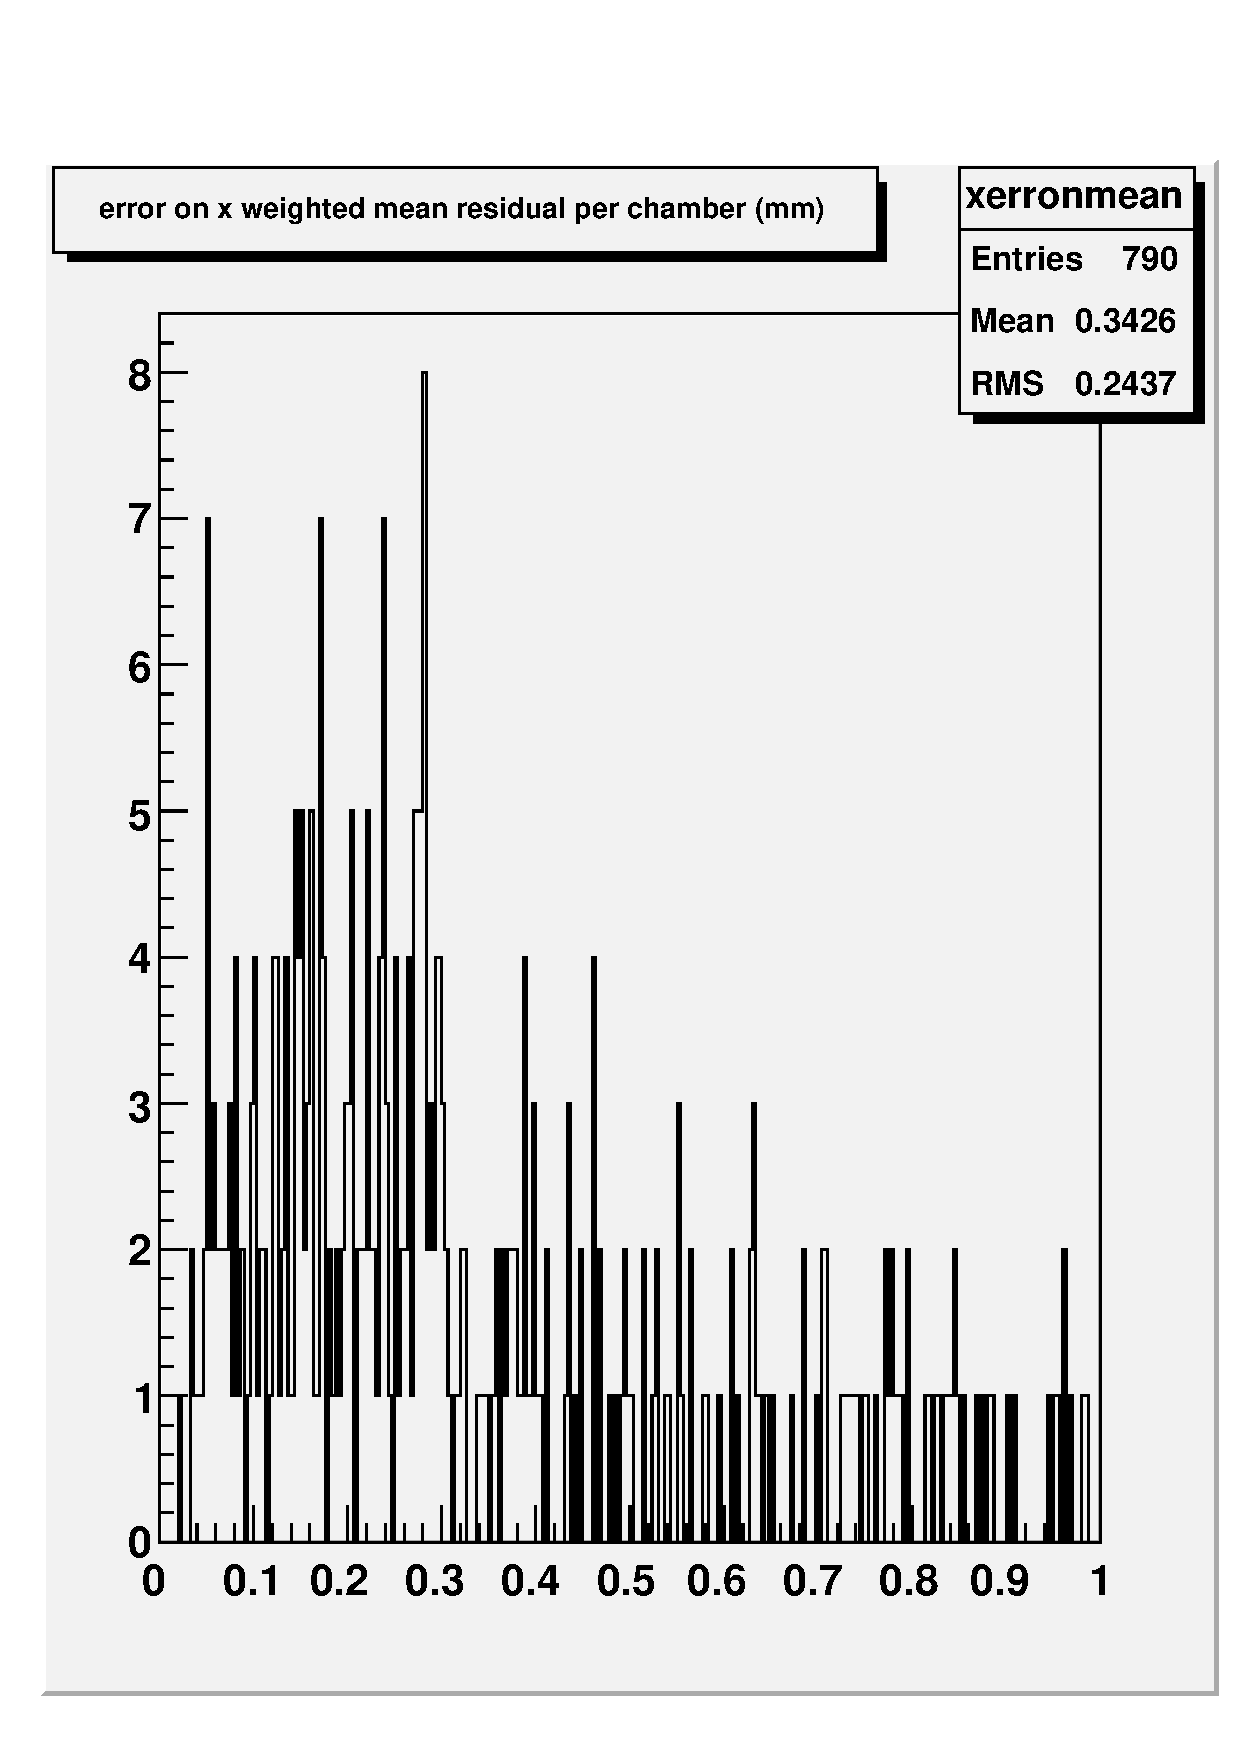
\includegraphics[width=\linewidth]{xerronmeanPT10.pdf}

\column{0.3\linewidth}
$p_T > 35$~GeV

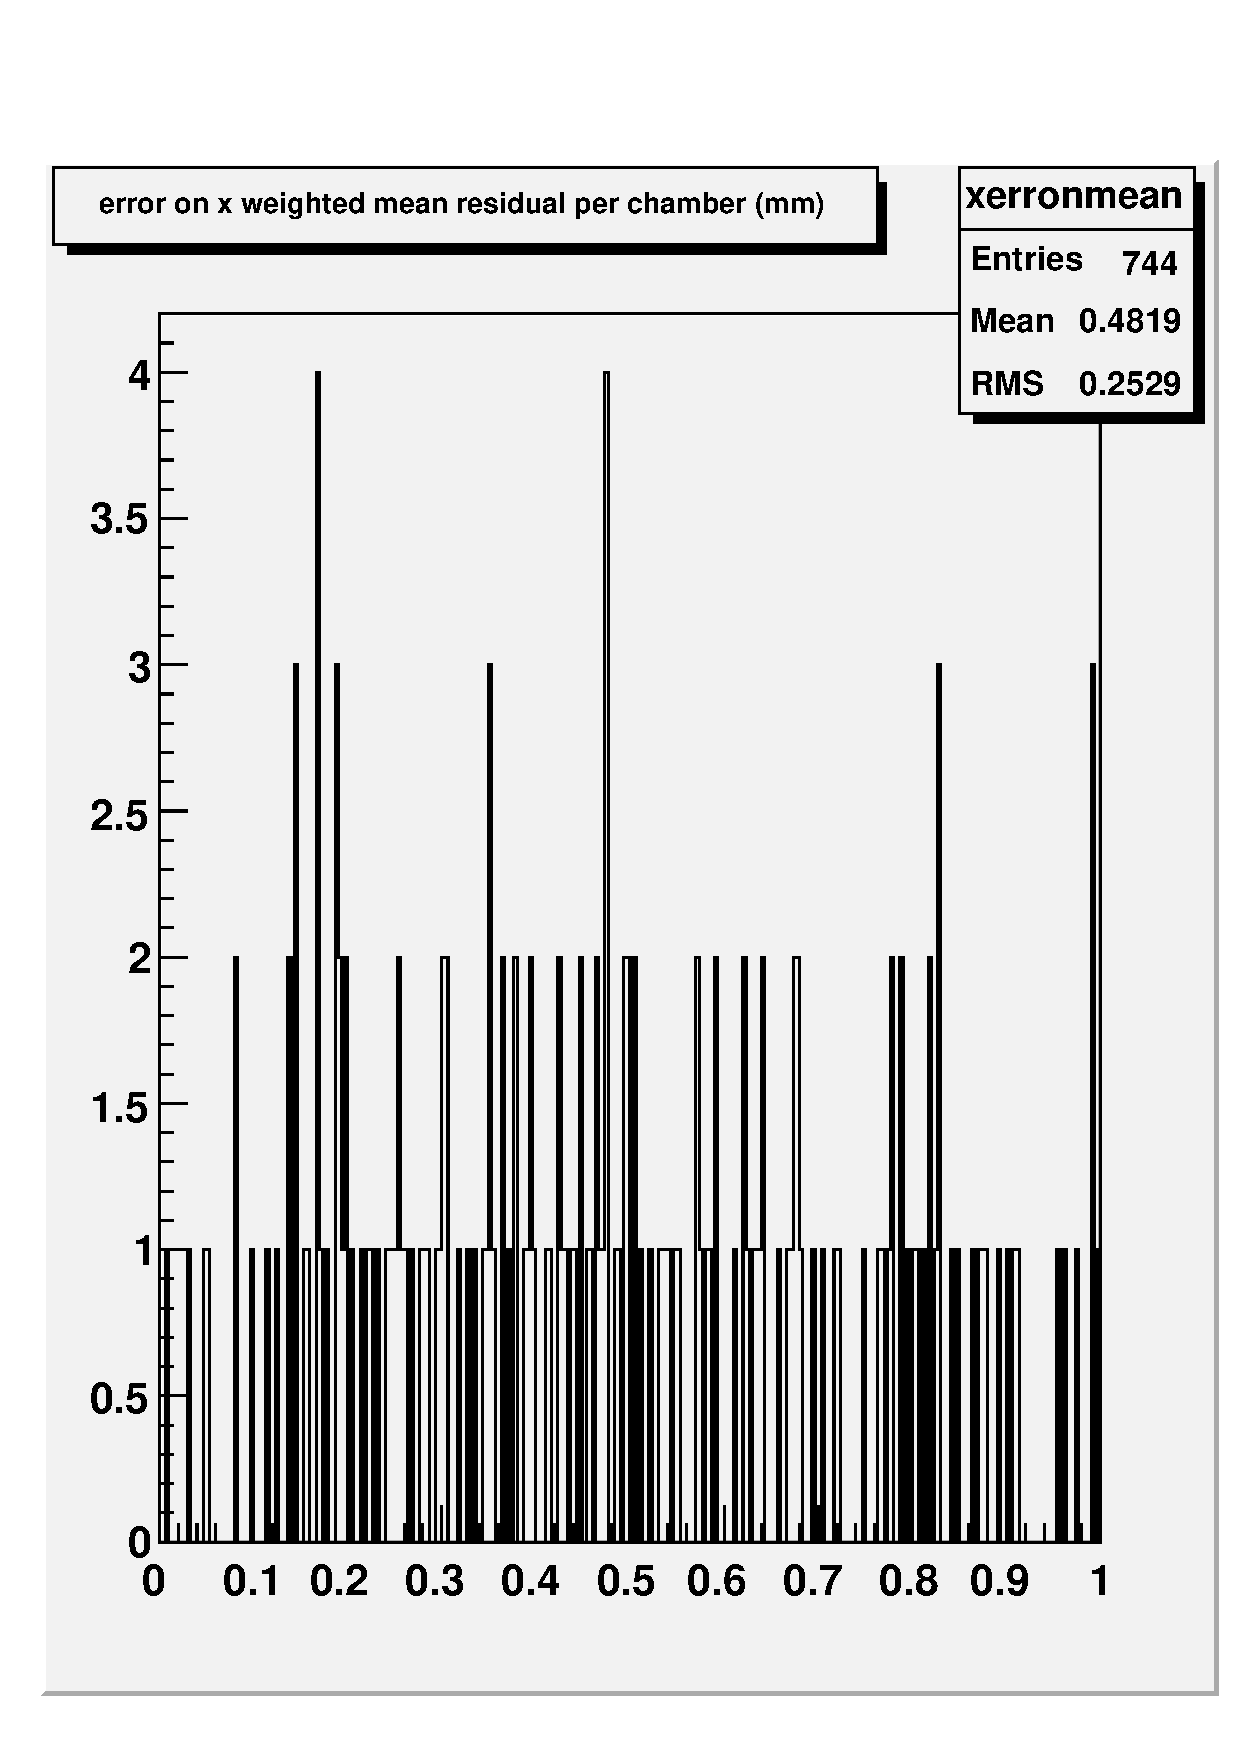
\includegraphics[width=\linewidth]{xerronmeanPT35.pdf}
\end{columns}
\end{center}

\end{frame}

\begin{frame}
\frametitle{Barrel \only<1>{aligned positions}\only<2>{track residuals}}

\only<1>{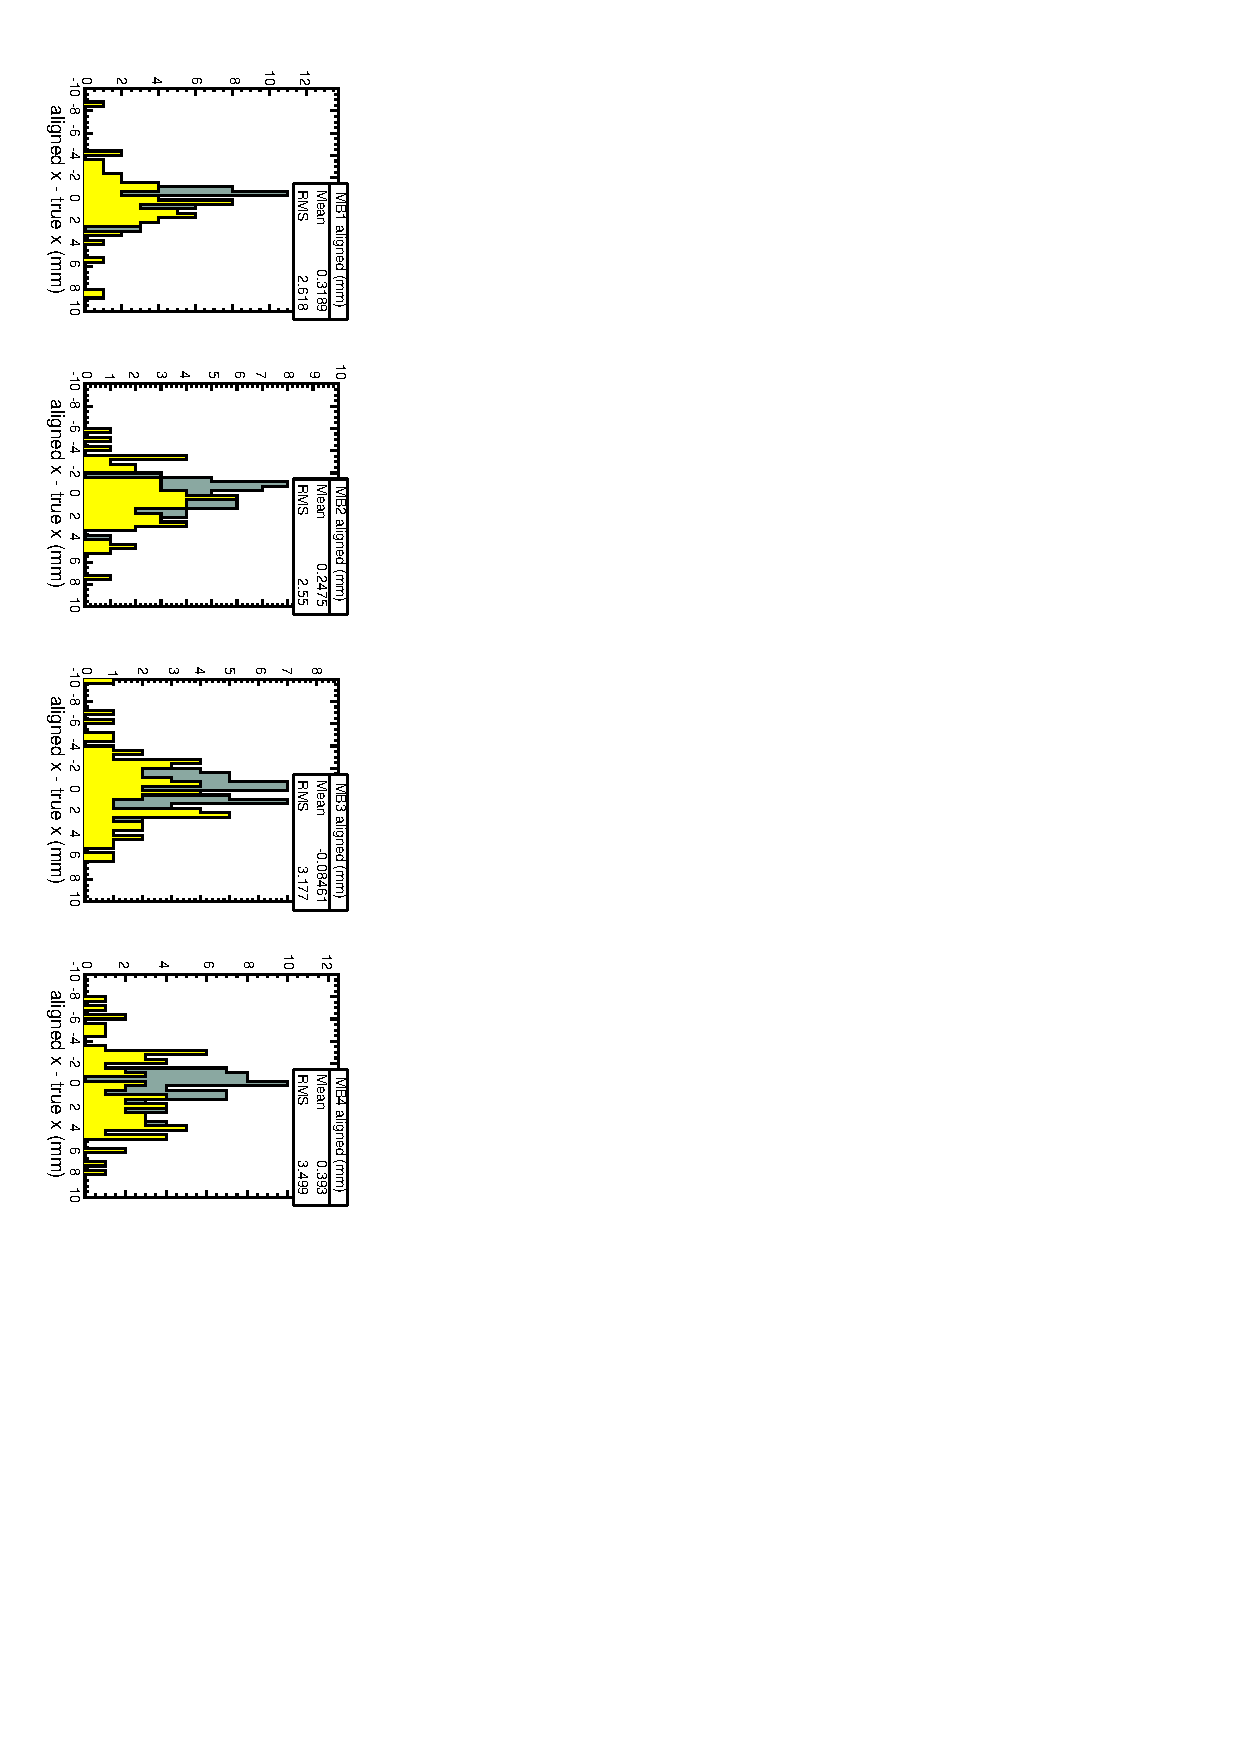
\includegraphics[height=\linewidth, angle=90]{S43_plots/RestrictPT10_MuonPT5_barrelx.pdf}}
\only<2>{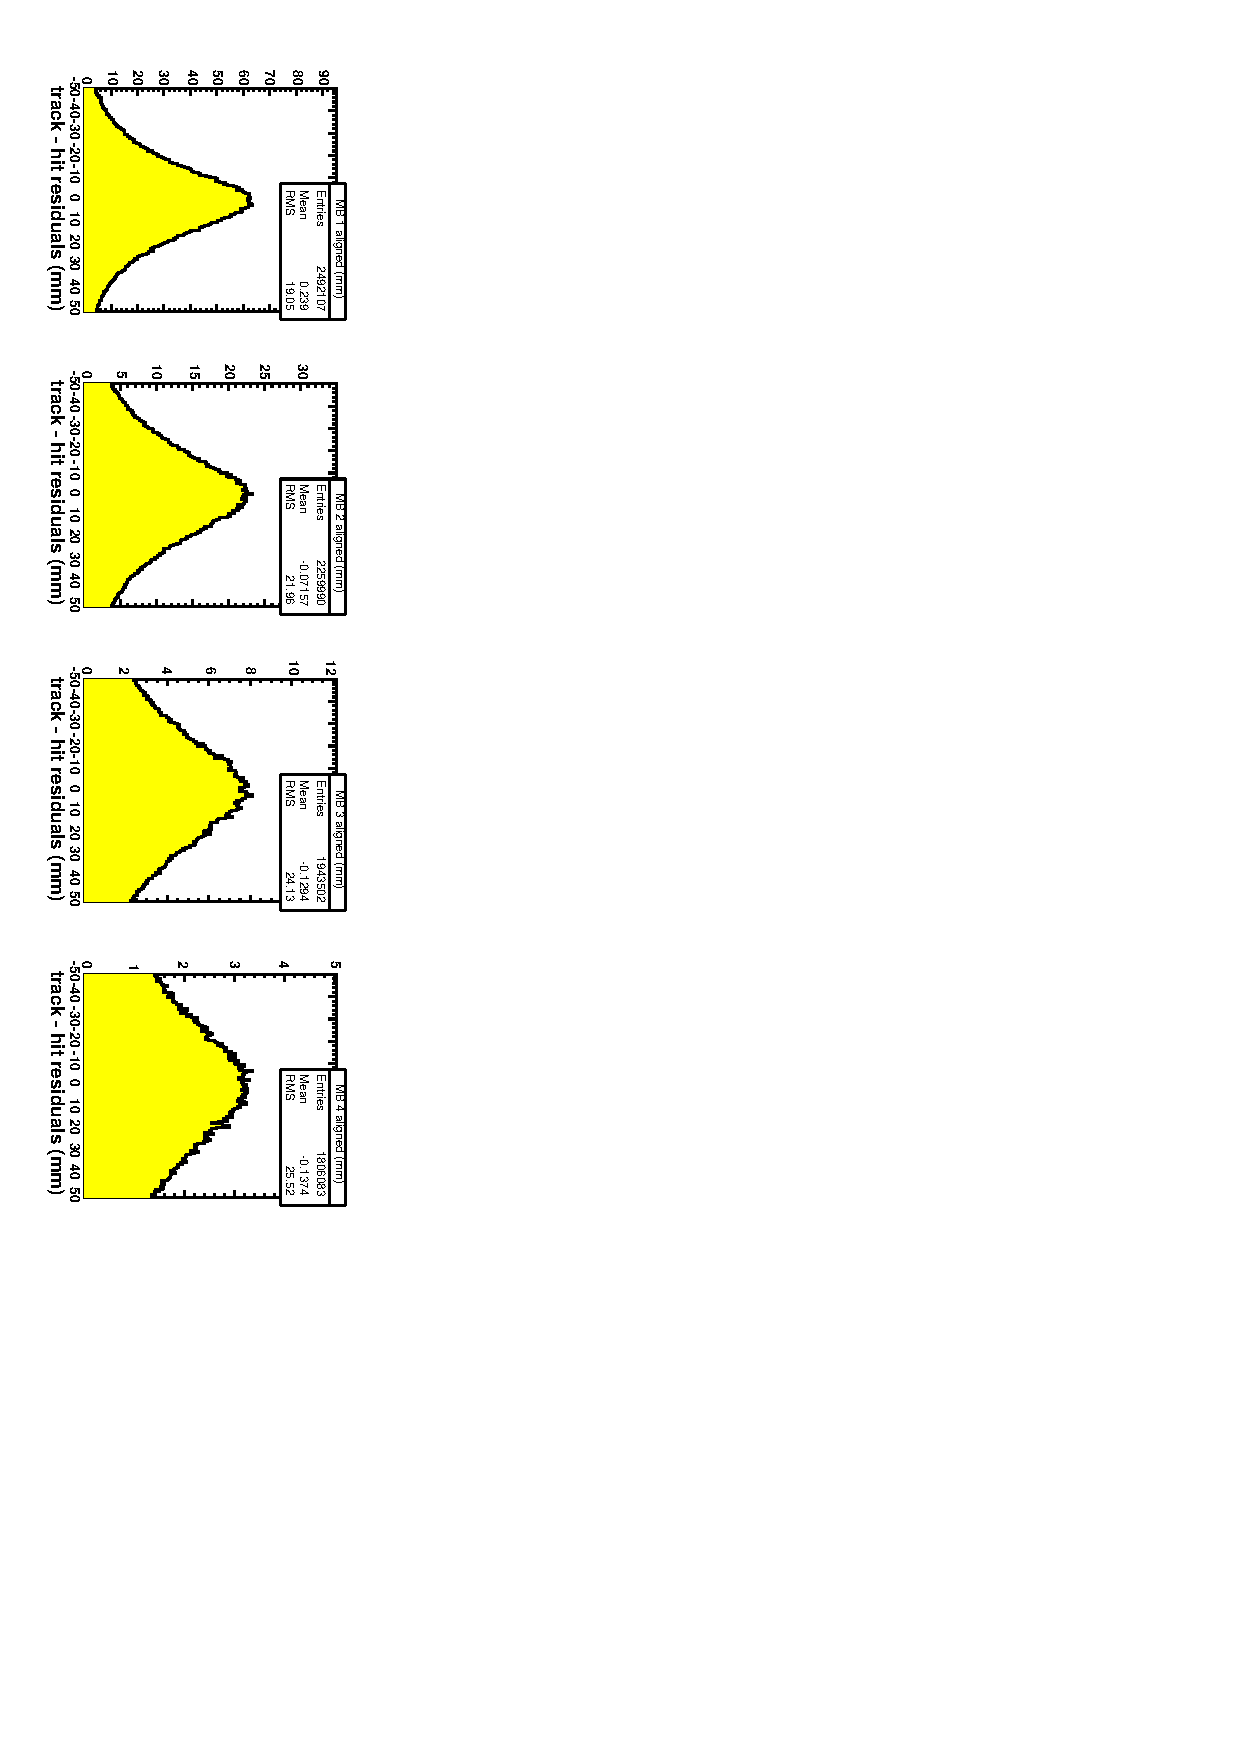
\includegraphics[height=\linewidth, angle=90]{S43_plots/RestrictPT10_MuonPT5_barrelresid.pdf}}

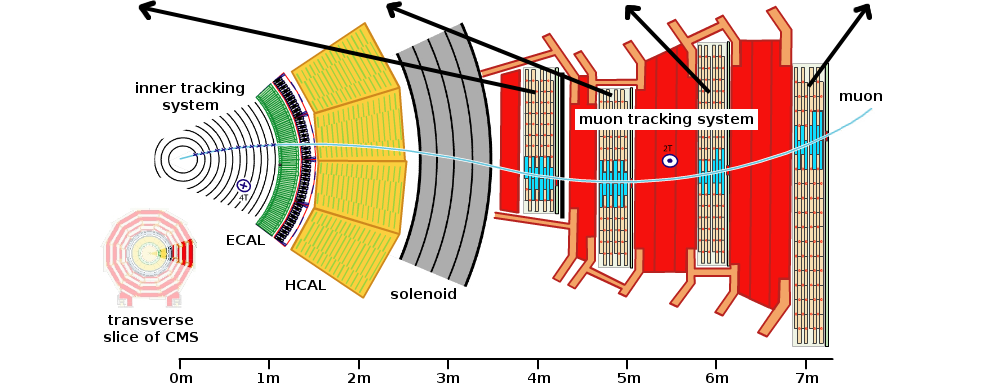
\includegraphics[width=\linewidth]{cms_slice.png}
\end{frame}

\begin{frame}
\frametitle{Barrel positions: $x$, $y$, $\phi_z$}

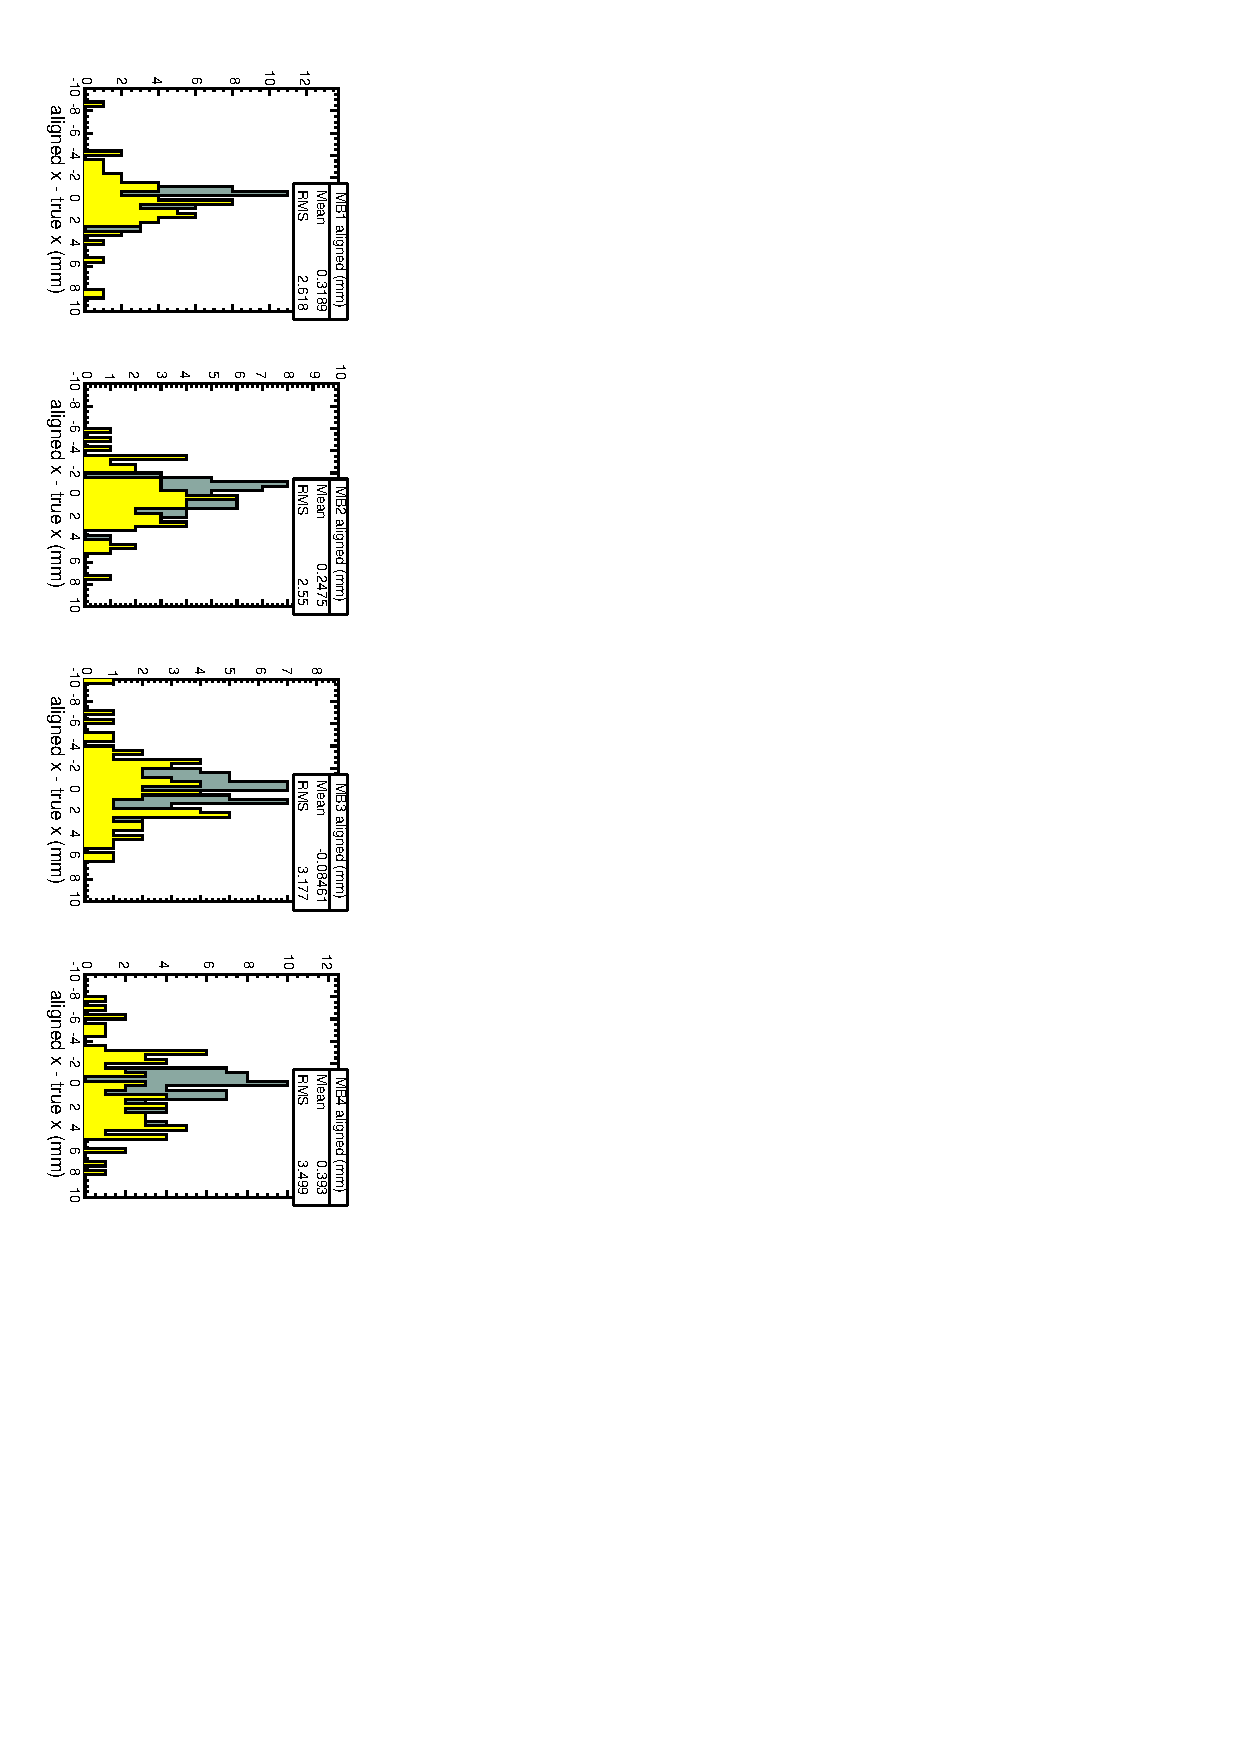
\includegraphics[height=\linewidth, angle=90]{S43_plots/RestrictPT10_MuonPT5_barrelx.pdf}

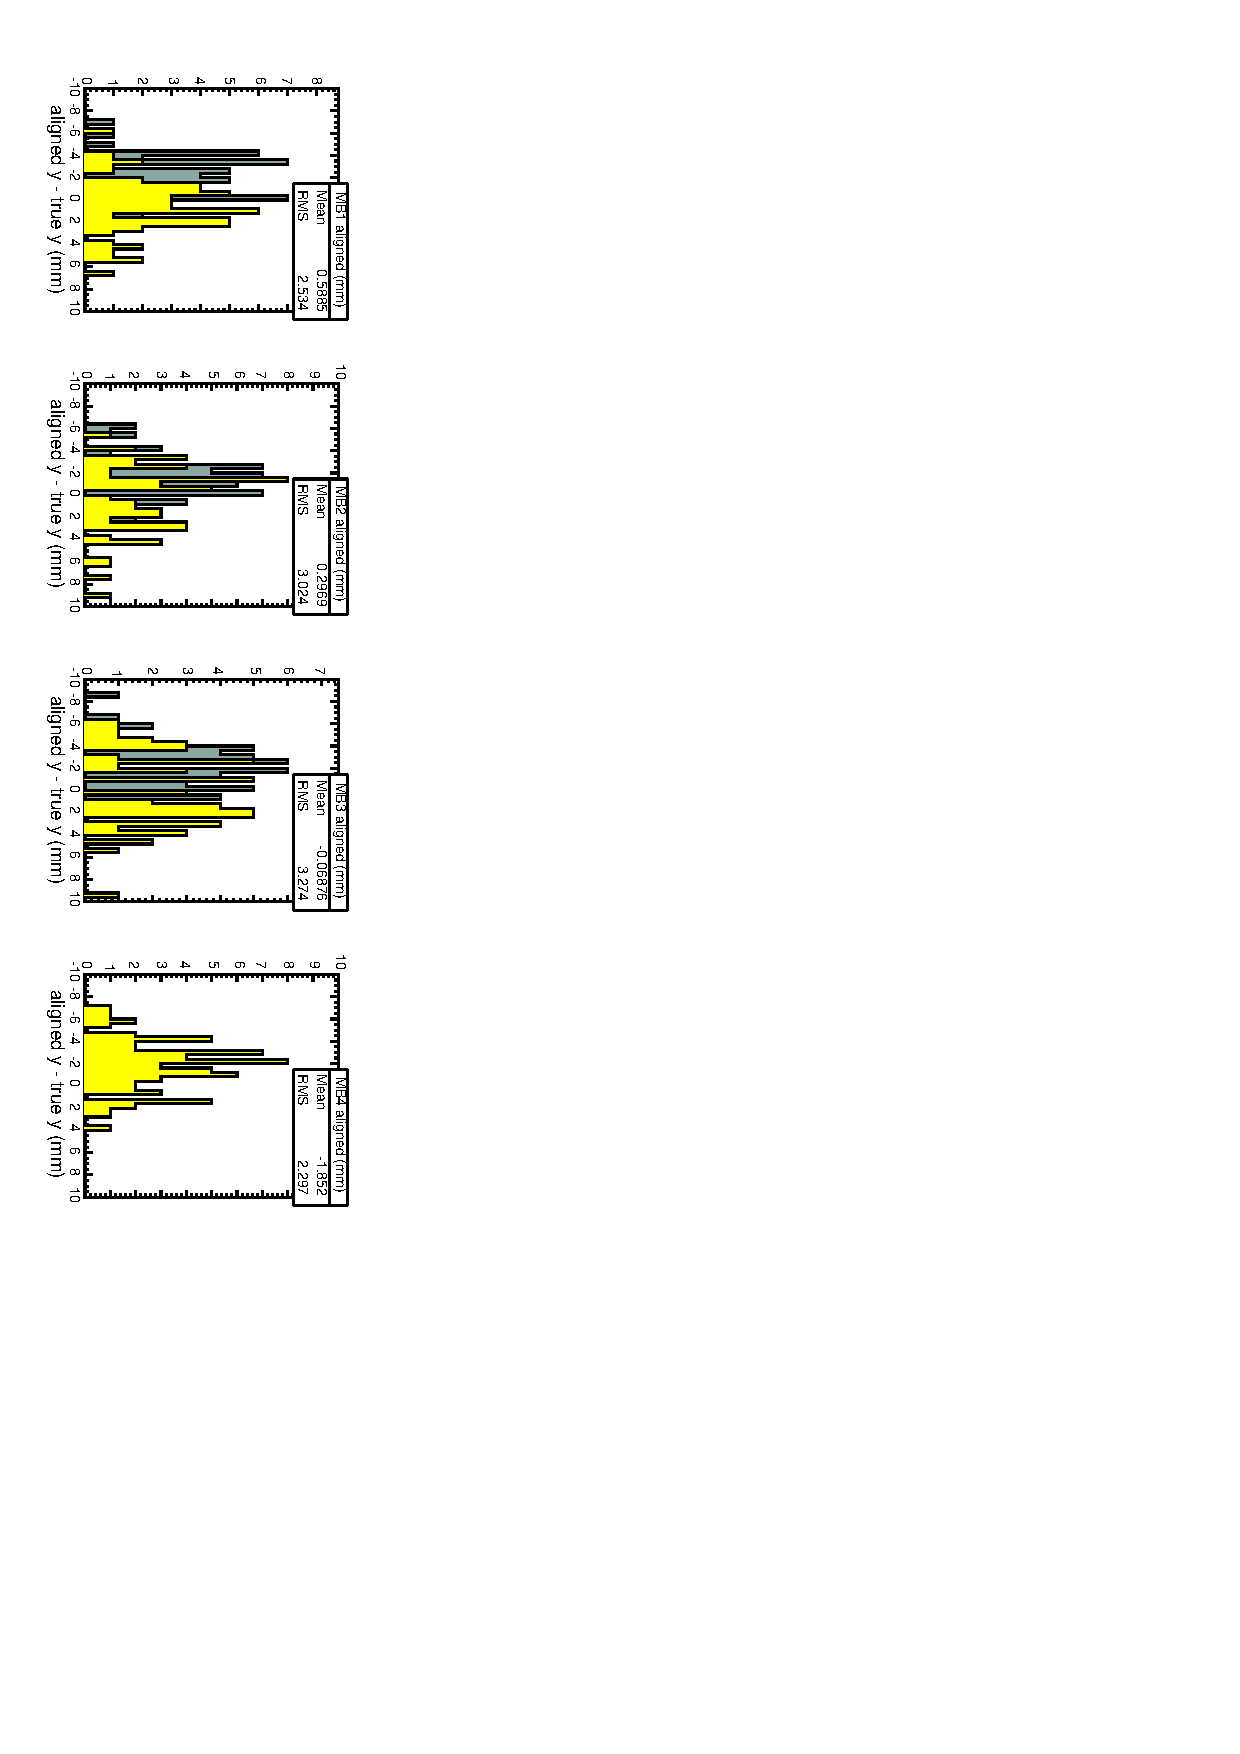
\includegraphics[height=\linewidth, angle=90]{S43_plots/RestrictPT10_MuonPT5_barrely.pdf}

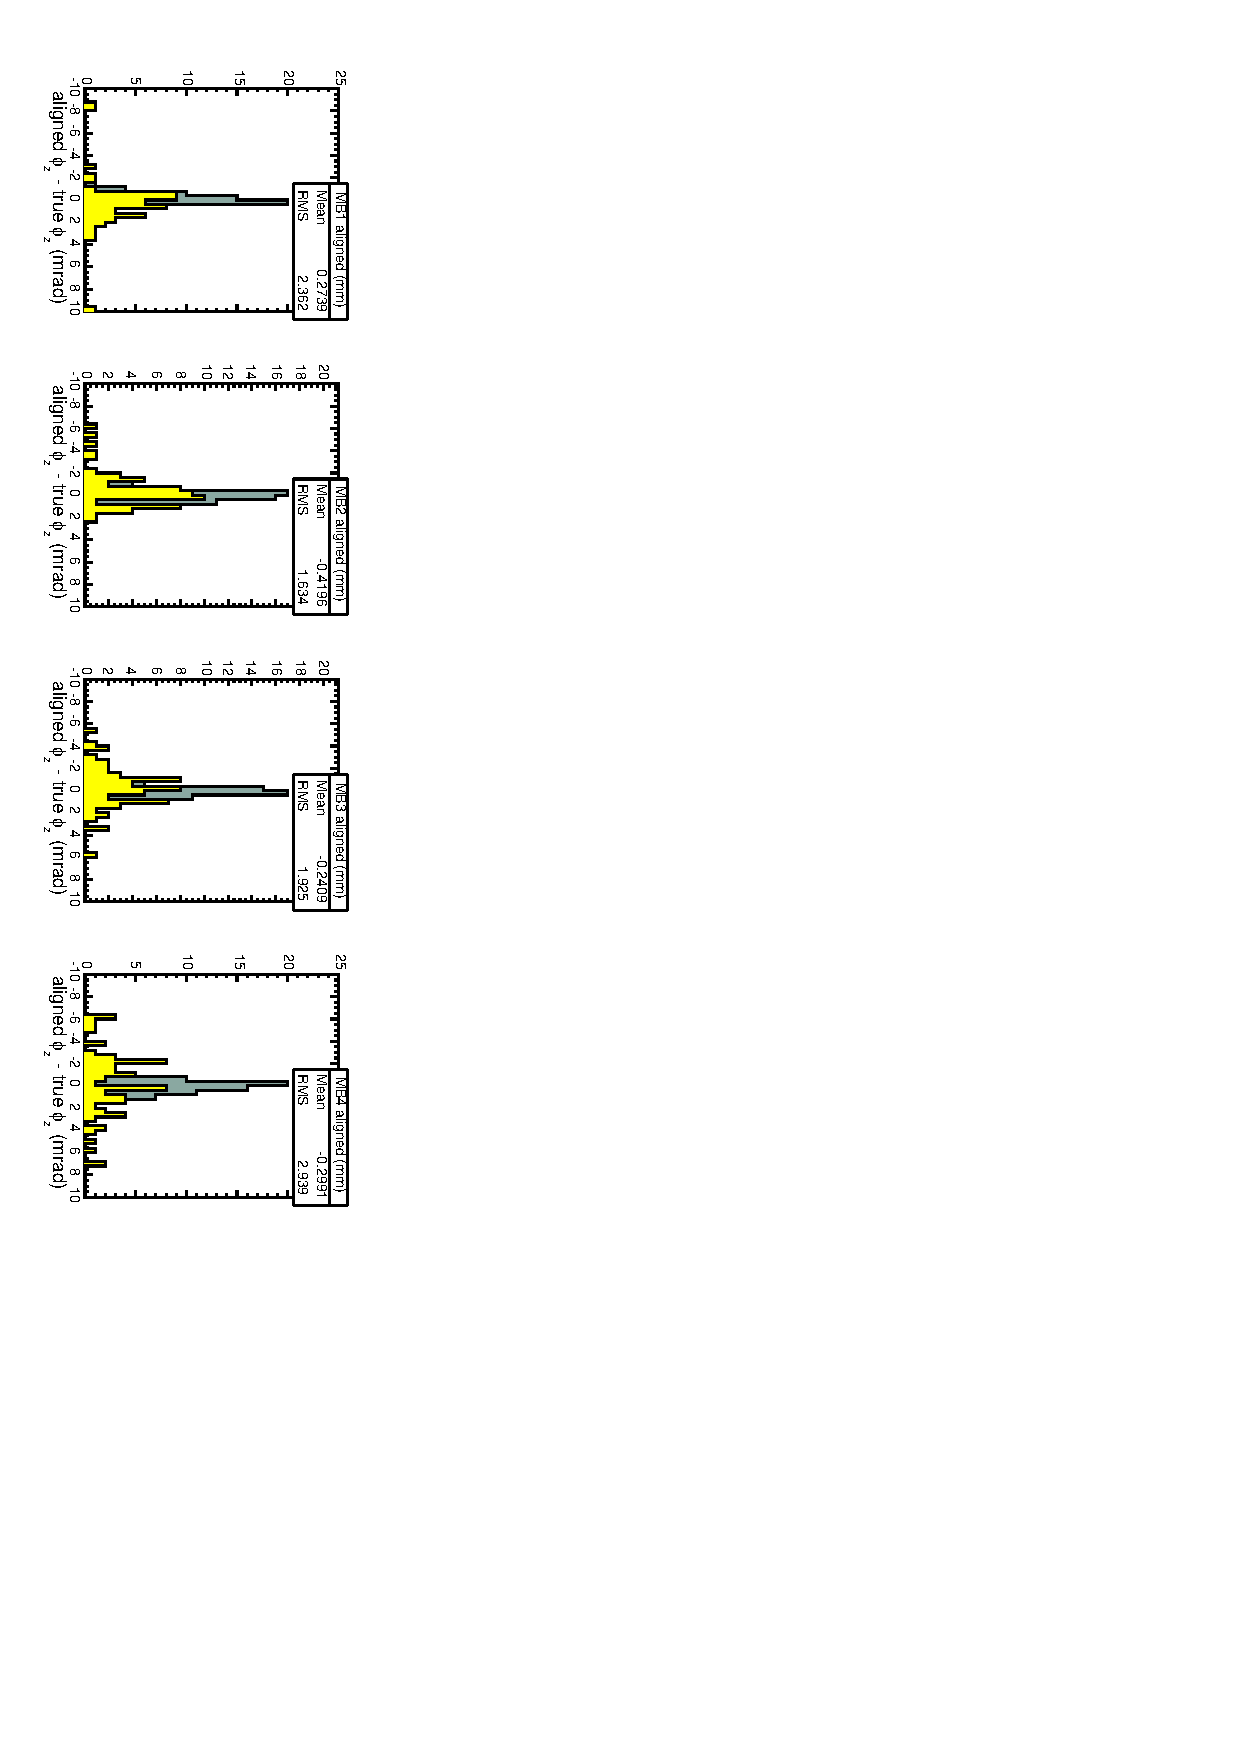
\includegraphics[height=\linewidth, angle=90]{S43_plots/RestrictPT10_MuonPT5_barrelphiz.pdf}

\end{frame}

\begin{frame}
\frametitle{Endcap \only<1>{aligned positions}\only<2>{track residuals}}

\begin{columns}
\column{0.35\linewidth}
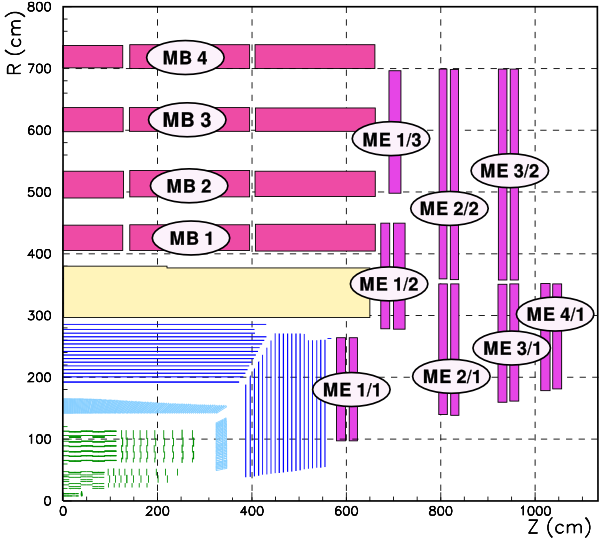
\includegraphics[width=\linewidth]{muon_system.png}
\column{0.8\linewidth}
\only<1>{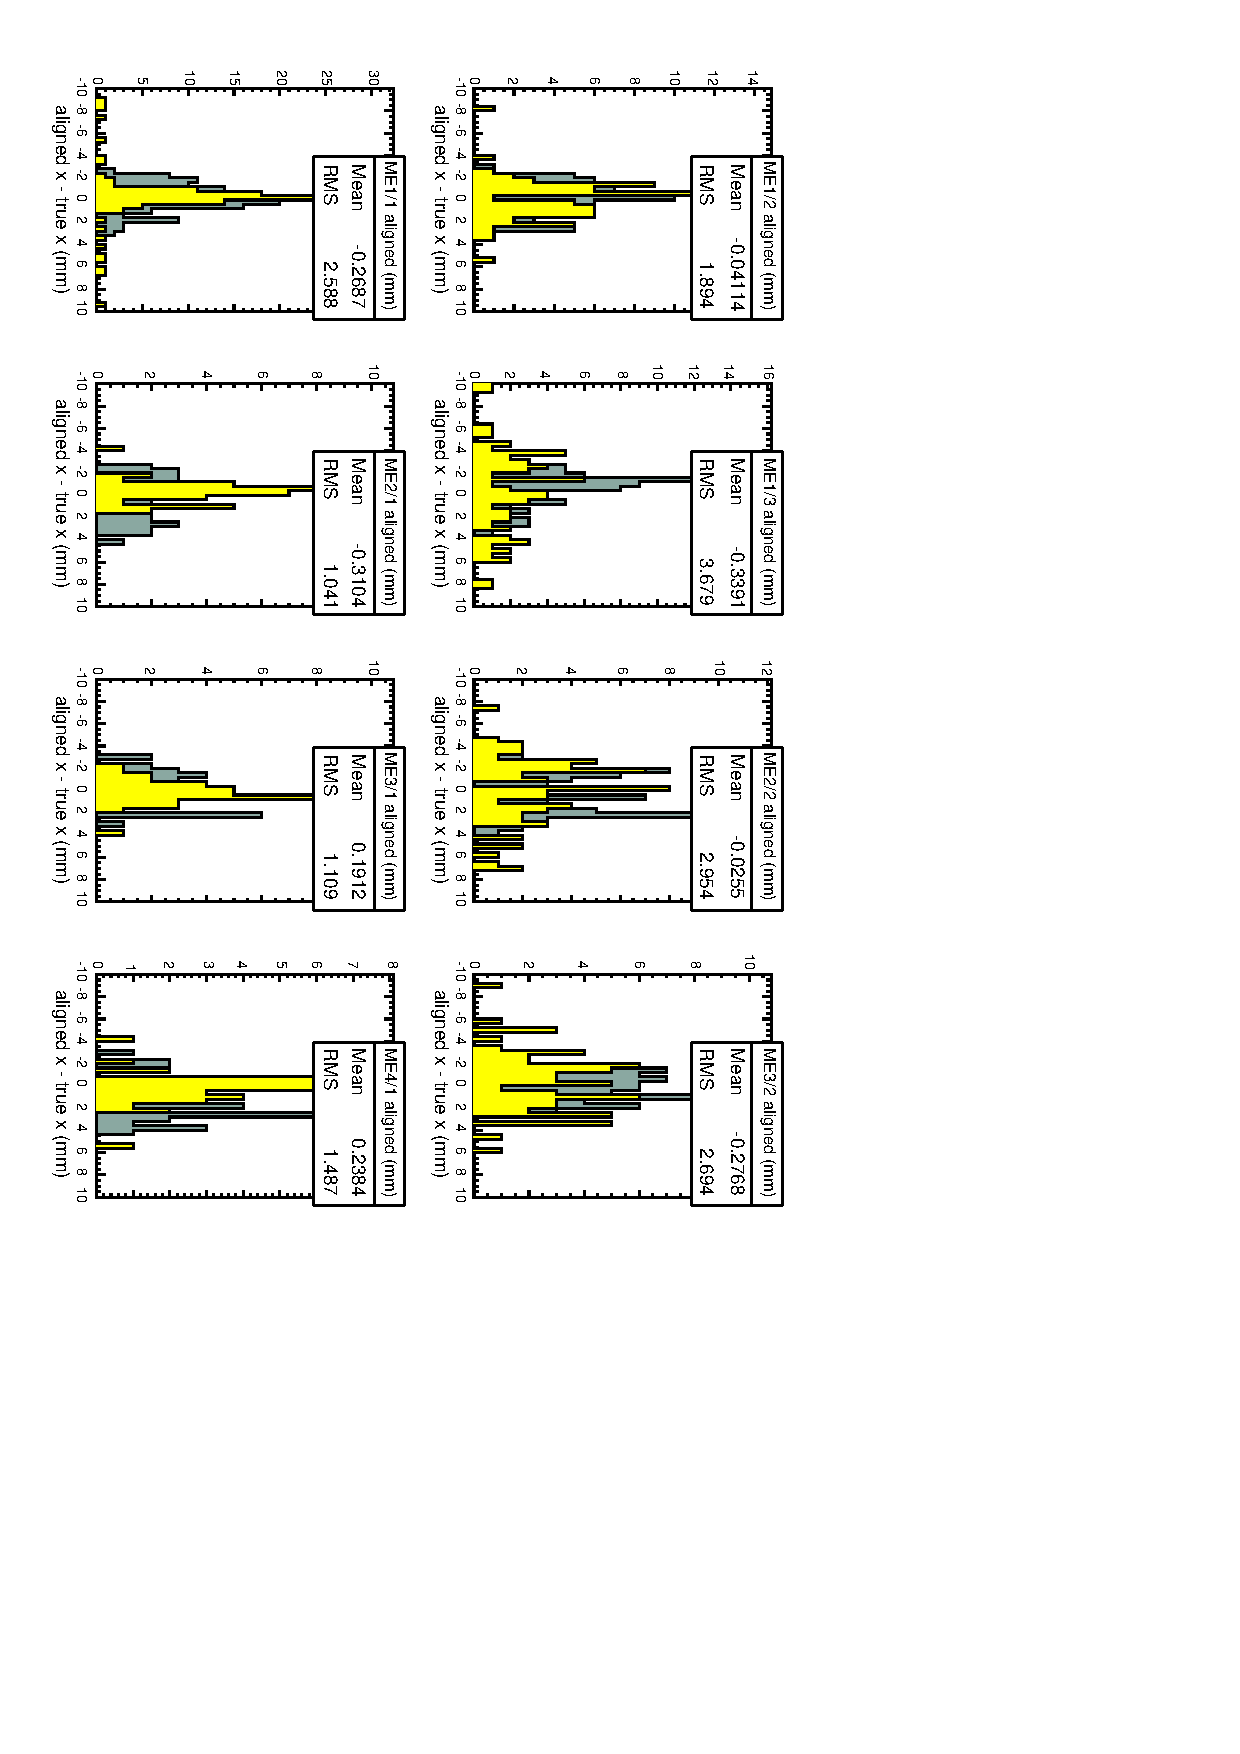
\includegraphics[height=\linewidth, angle=90]{S43_plots/RestrictPT10_MuonPT5_endcapx.pdf}}
\only<2>{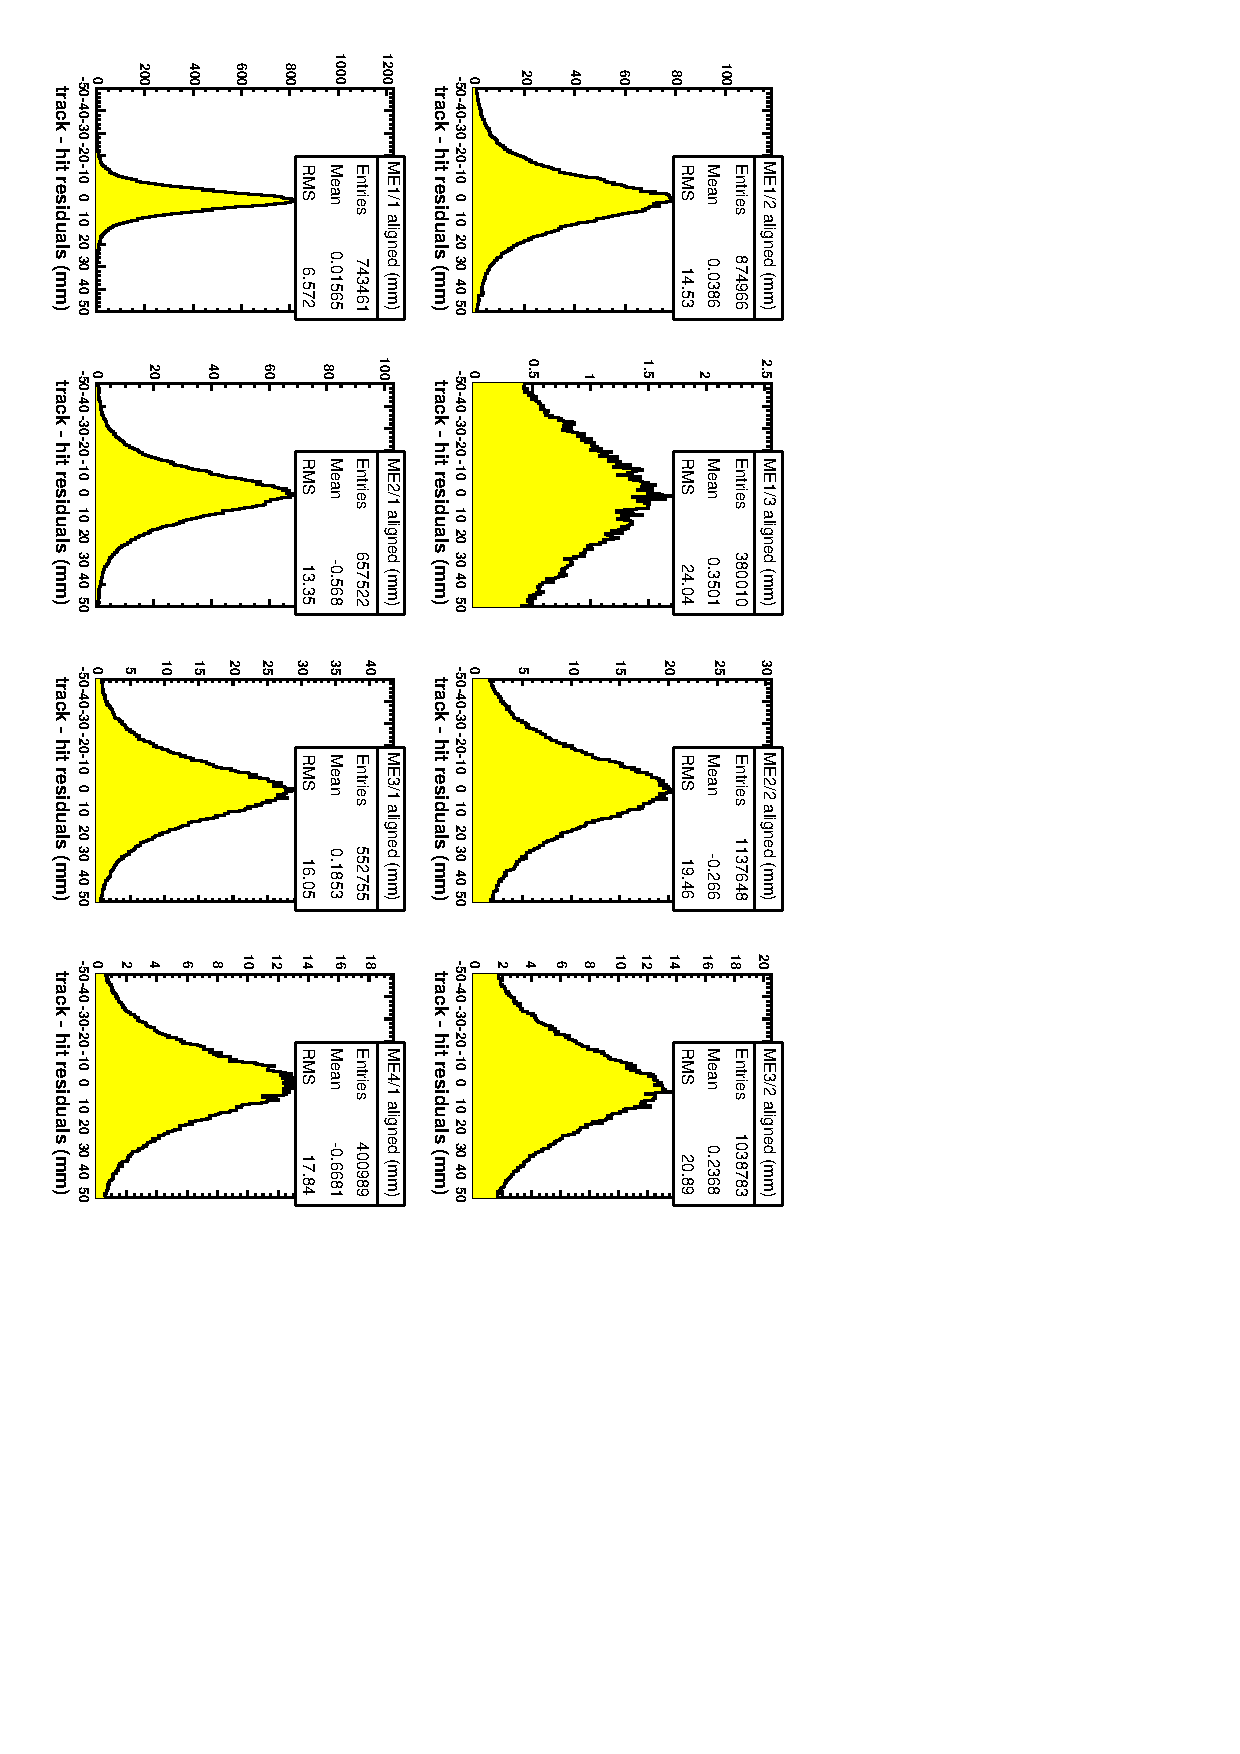
\includegraphics[height=\linewidth, angle=90]{S43_plots/RestrictPT10_MuonPT5_endcapresid.pdf}}
\end{columns}

\end{frame}

\begin{frame}
\frametitle{Endcap positions: \only<1>{$y$}\only<2>{$\phi_z$}}
\only<1>{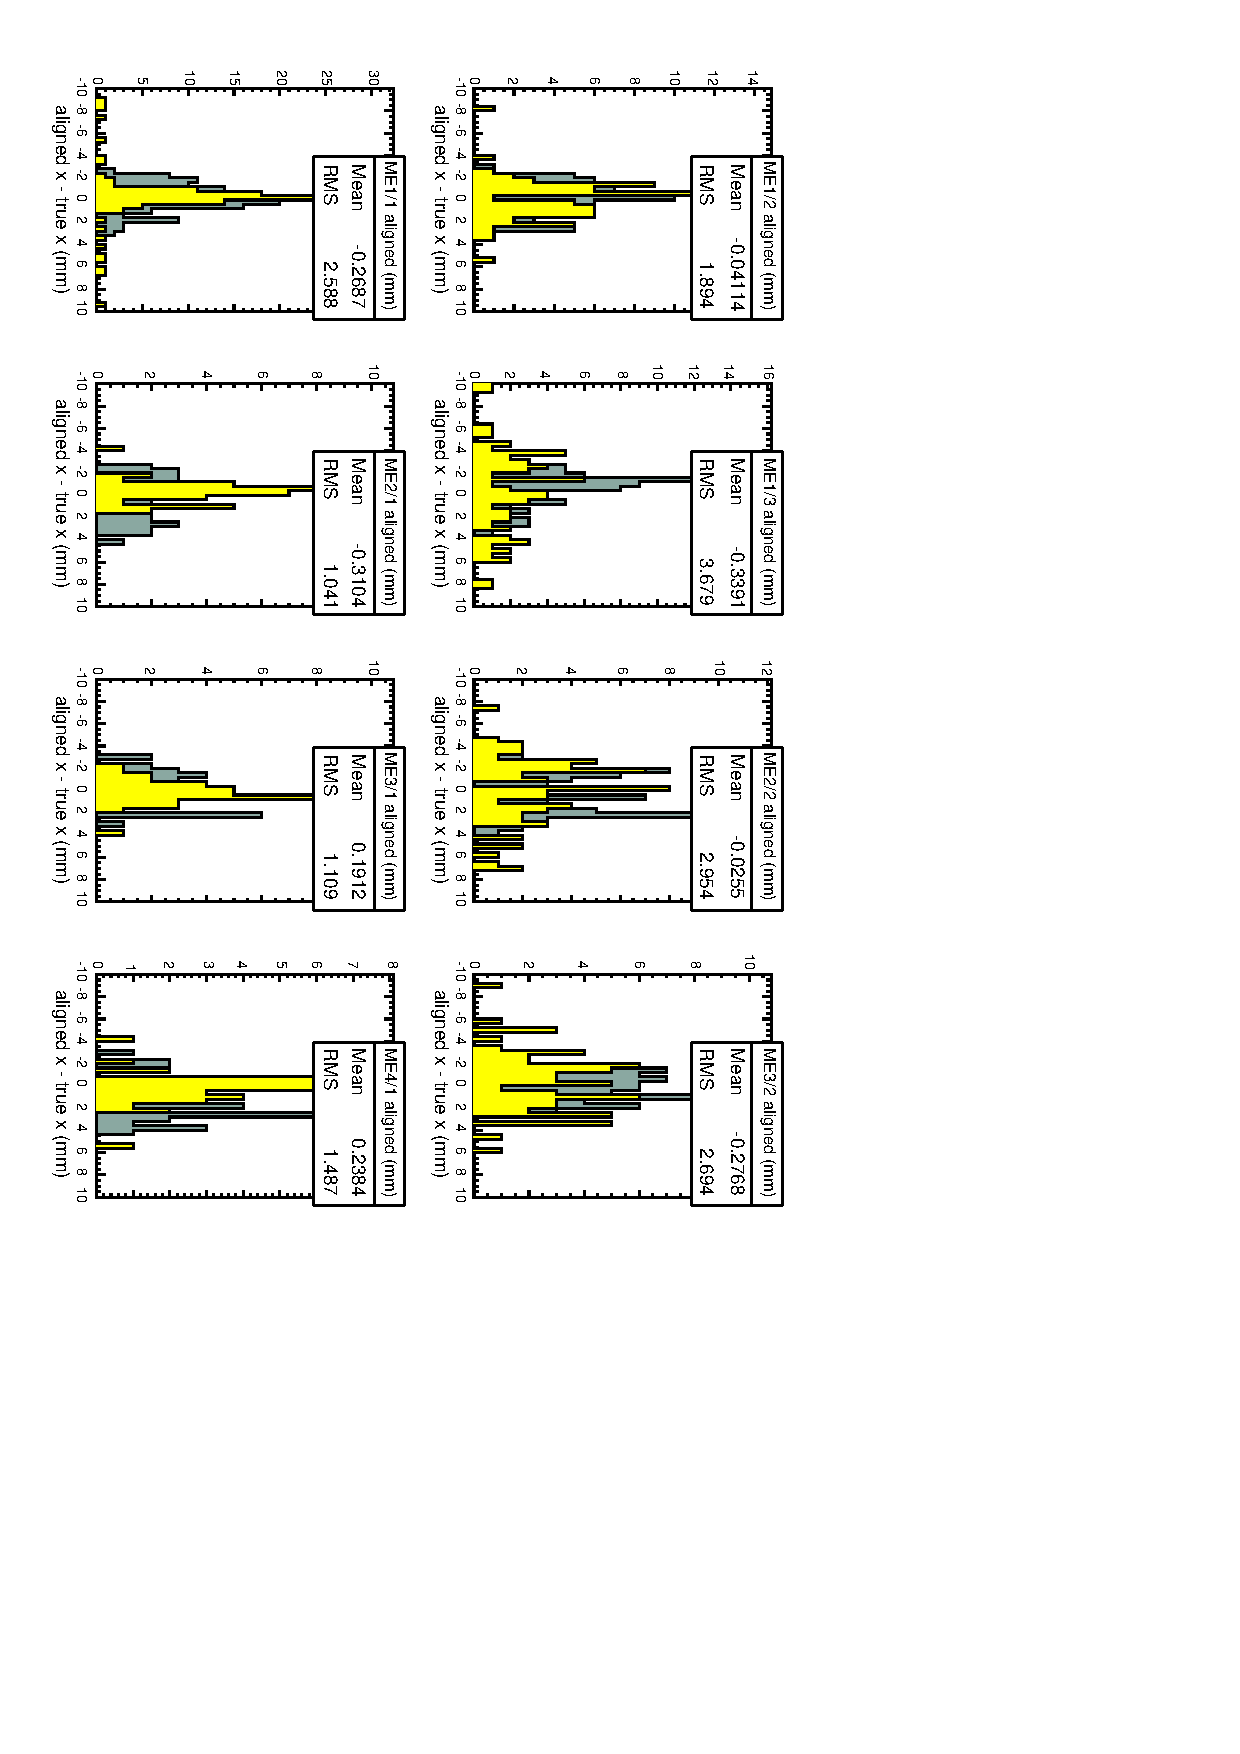
\includegraphics[height=\linewidth, angle=90]{S43_plots/RestrictPT10_MuonPT5_endcapy.pdf}}
\only<2>{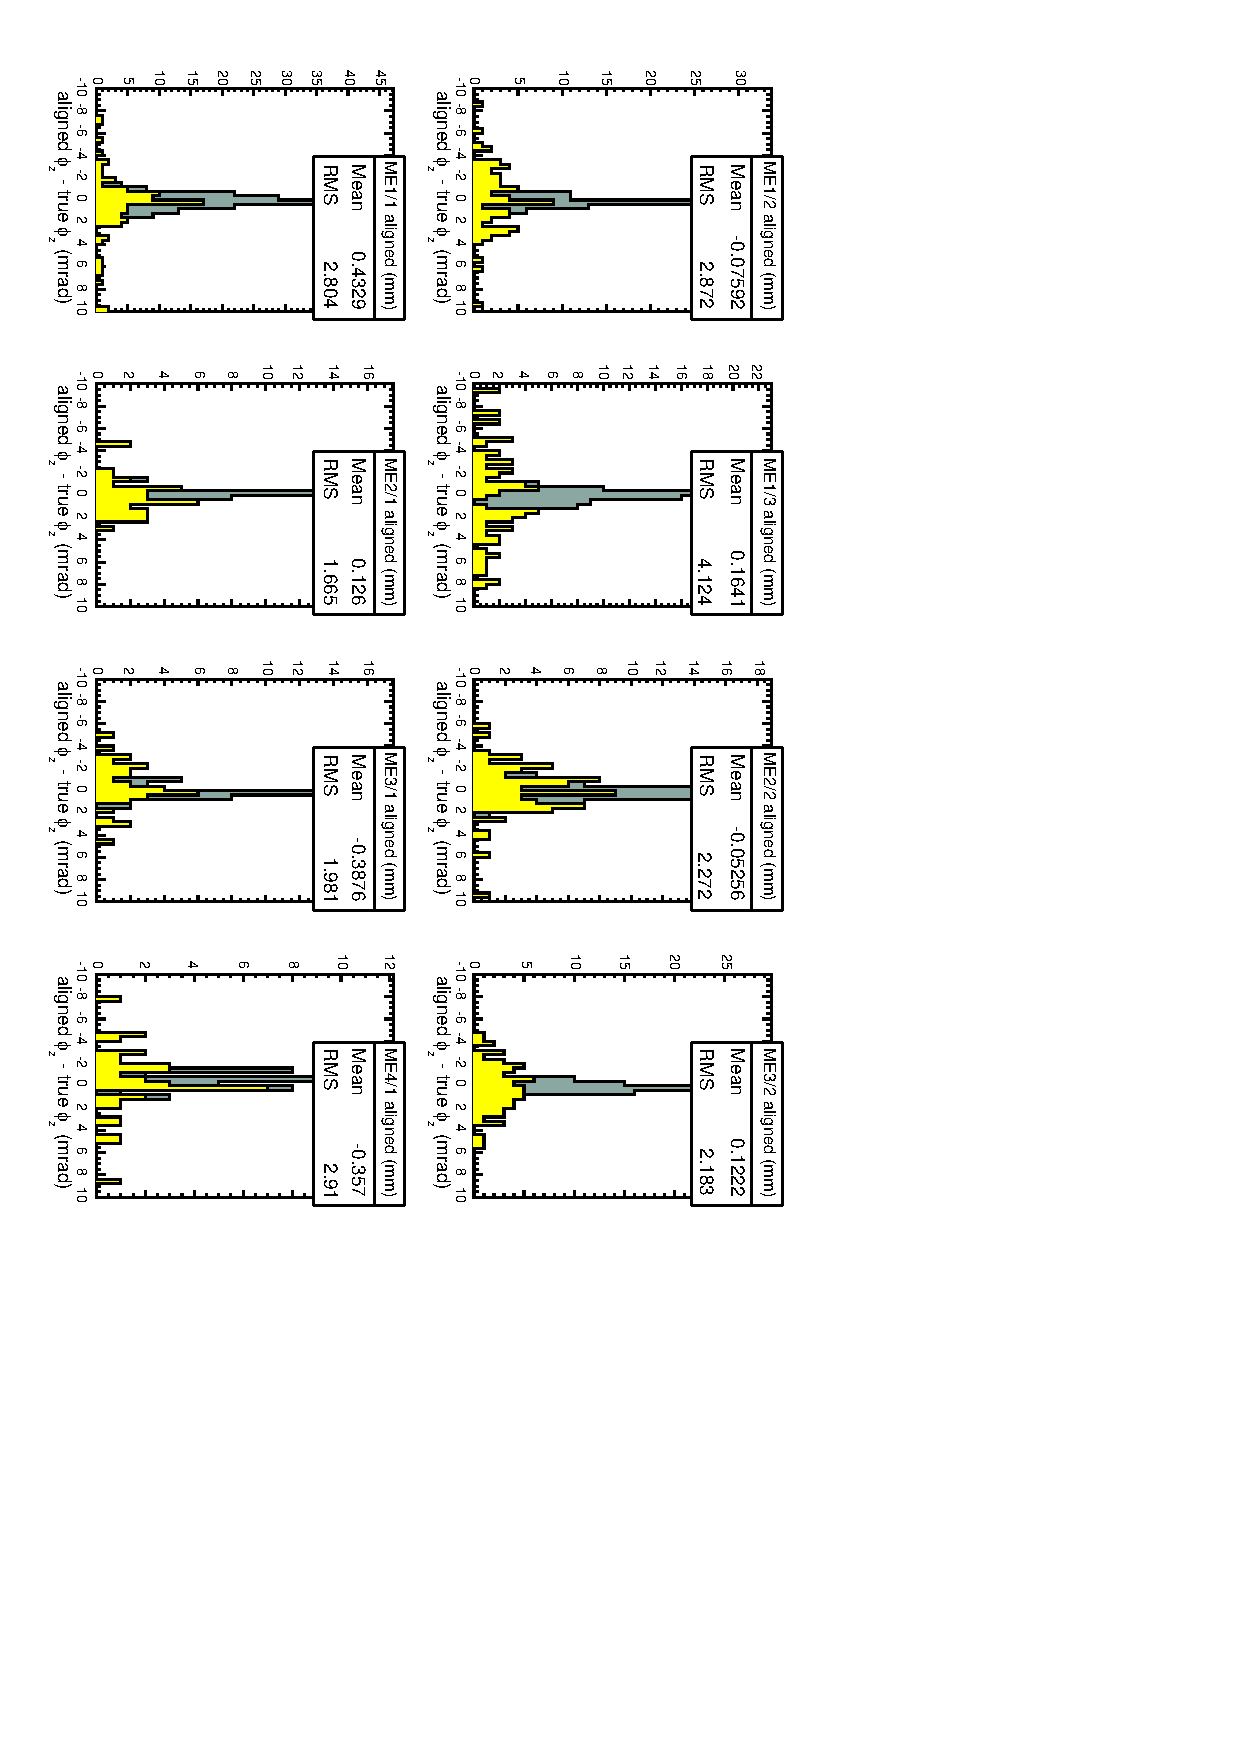
\includegraphics[height=\linewidth, angle=90]{S43_plots/RestrictPT10_MuonPT5_endcapphiz.pdf}}
\end{frame}

\begin{frame}
\frametitle{Regrets}

\begin{itemize}
\item We have a tool for selecting aligned chambers by hand: I would have selected MB1, ME1/1, ME1/2, ME2/1, ME2/2, ME3/1
\item Discovered a bug in handling of angles, so we didn't use it
\end{itemize}

\vfill
\hspace{-0.83 cm} \textcolor{darkblue}{\Large Software to-do list}
\begin{itemize}
\item Fix geometry-merging tool
\item Implement selection: take only chambers with $\mbox{stdev}/\sqrt{N}$ $<$ 1~mm
\item Make tracker $\chi^2$ and DOF cuts formal (selection module)
\item APE of hits is $\sqrt{2}$ larger than what is applied in configuration file!
\item Update monitoring plots in CVS
\end{itemize}

\end{frame}

\begin{frame}
\frametitle{GlobalMuon reconstruction: $Z'$}

\begin{itemize}
\item \textcolor{black}{initial constants}
\item \textcolor{red}{HIP tracks-only alignment}
\item \textcolor{blue}{MillePede-survey in barrel, HIP in endcap}
\end{itemize}

\begin{center}
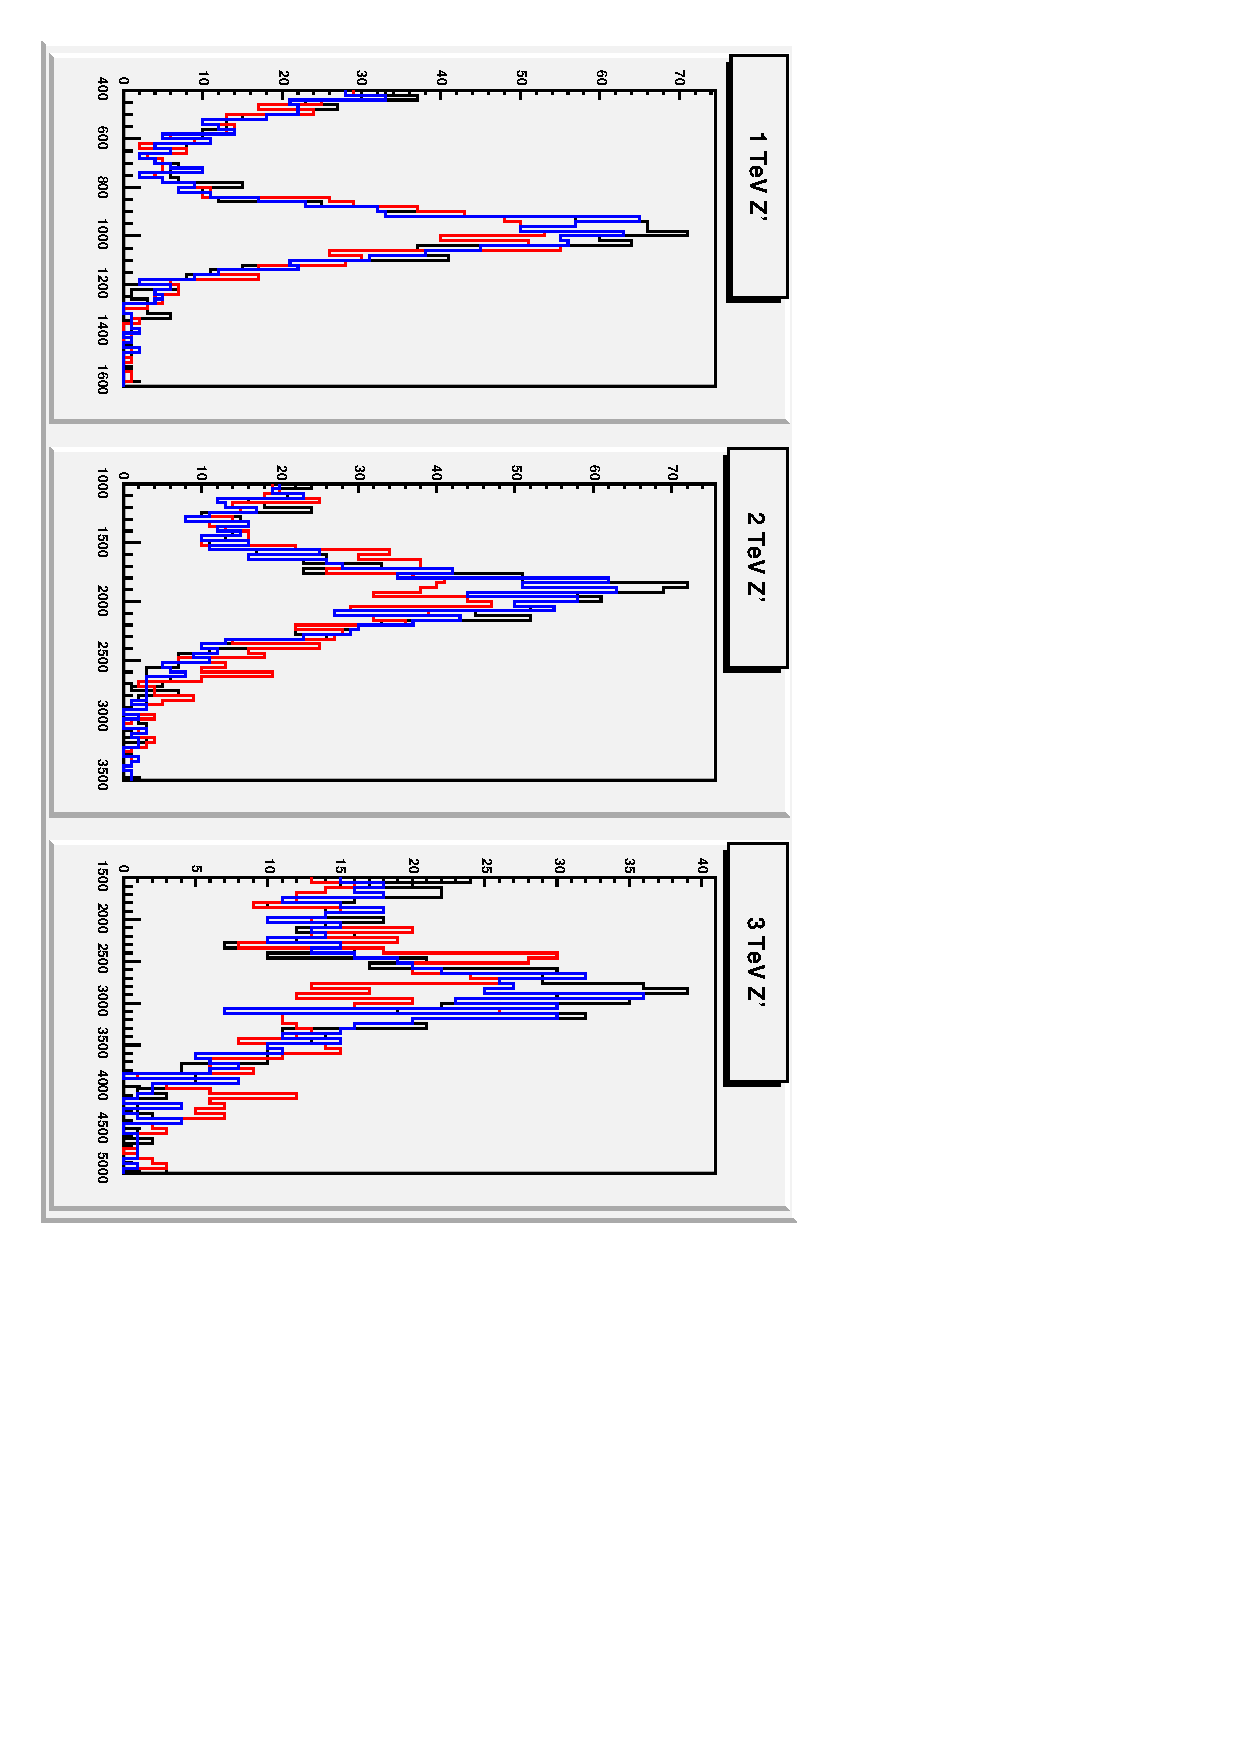
\includegraphics[height=0.9\linewidth, angle=90]{zprime_mass.pdf}
\end{center}
\end{frame}

\begin{frame}
\frametitle{Should we use it?}

Use MillePede-survey for the barrel, tracks-only for the endcap

\begin{itemize}\setlength{\itemsep}{0.25 cm}
\item endcap alignment (especially inner ring) is better than barrel because of statistics
\item if we only had 1~pb$^{-1}$ of real data, we would rely heavily on survey information (Muon0invPbScenario = Muon1invPbScenario)
\end{itemize}

\vfill
On the other hand\ldots
\begin{itemize}\setlength{\itemsep}{0.25 cm}
\item it means we worsen the resolution relative to 0~pb$^{-1}$ scenario
\item the MillePede-survey result is effectively a scenario like the
0~pb$^{-1}$ scenario, but with updated constants
\end{itemize}

\vfill
\hspace{-0.83 cm} \textcolor{darkblue}{\Large Conclusions}

\vfill Nevertheless, a very useful exercise, and we'll be using these event samples for more detector studies!

\label{numpages}
\end{frame}

\begin{frame}
\frametitle{MillePede-survey: $x$, $y$, $\phi_z$}

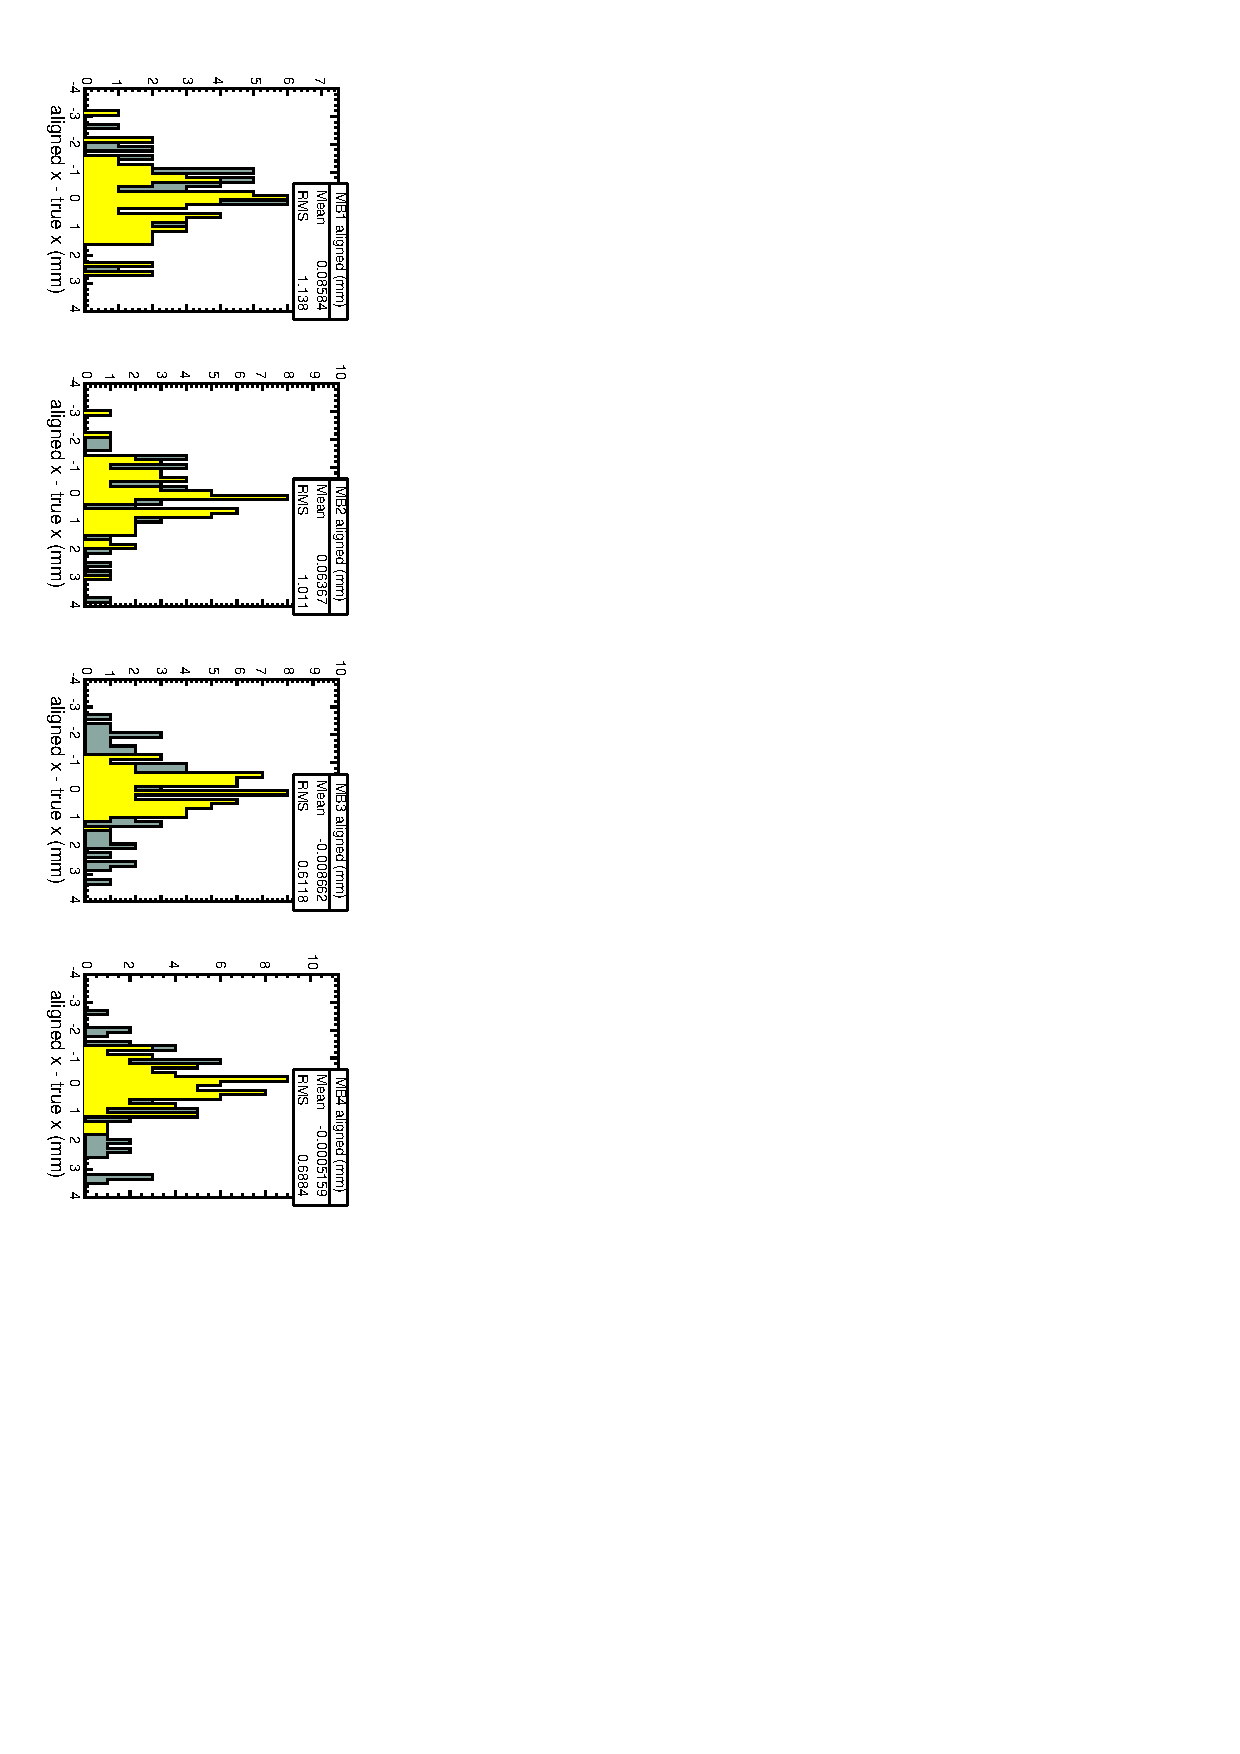
\includegraphics[height=\linewidth, angle=90]{S43_plots/MillePede_x.pdf}

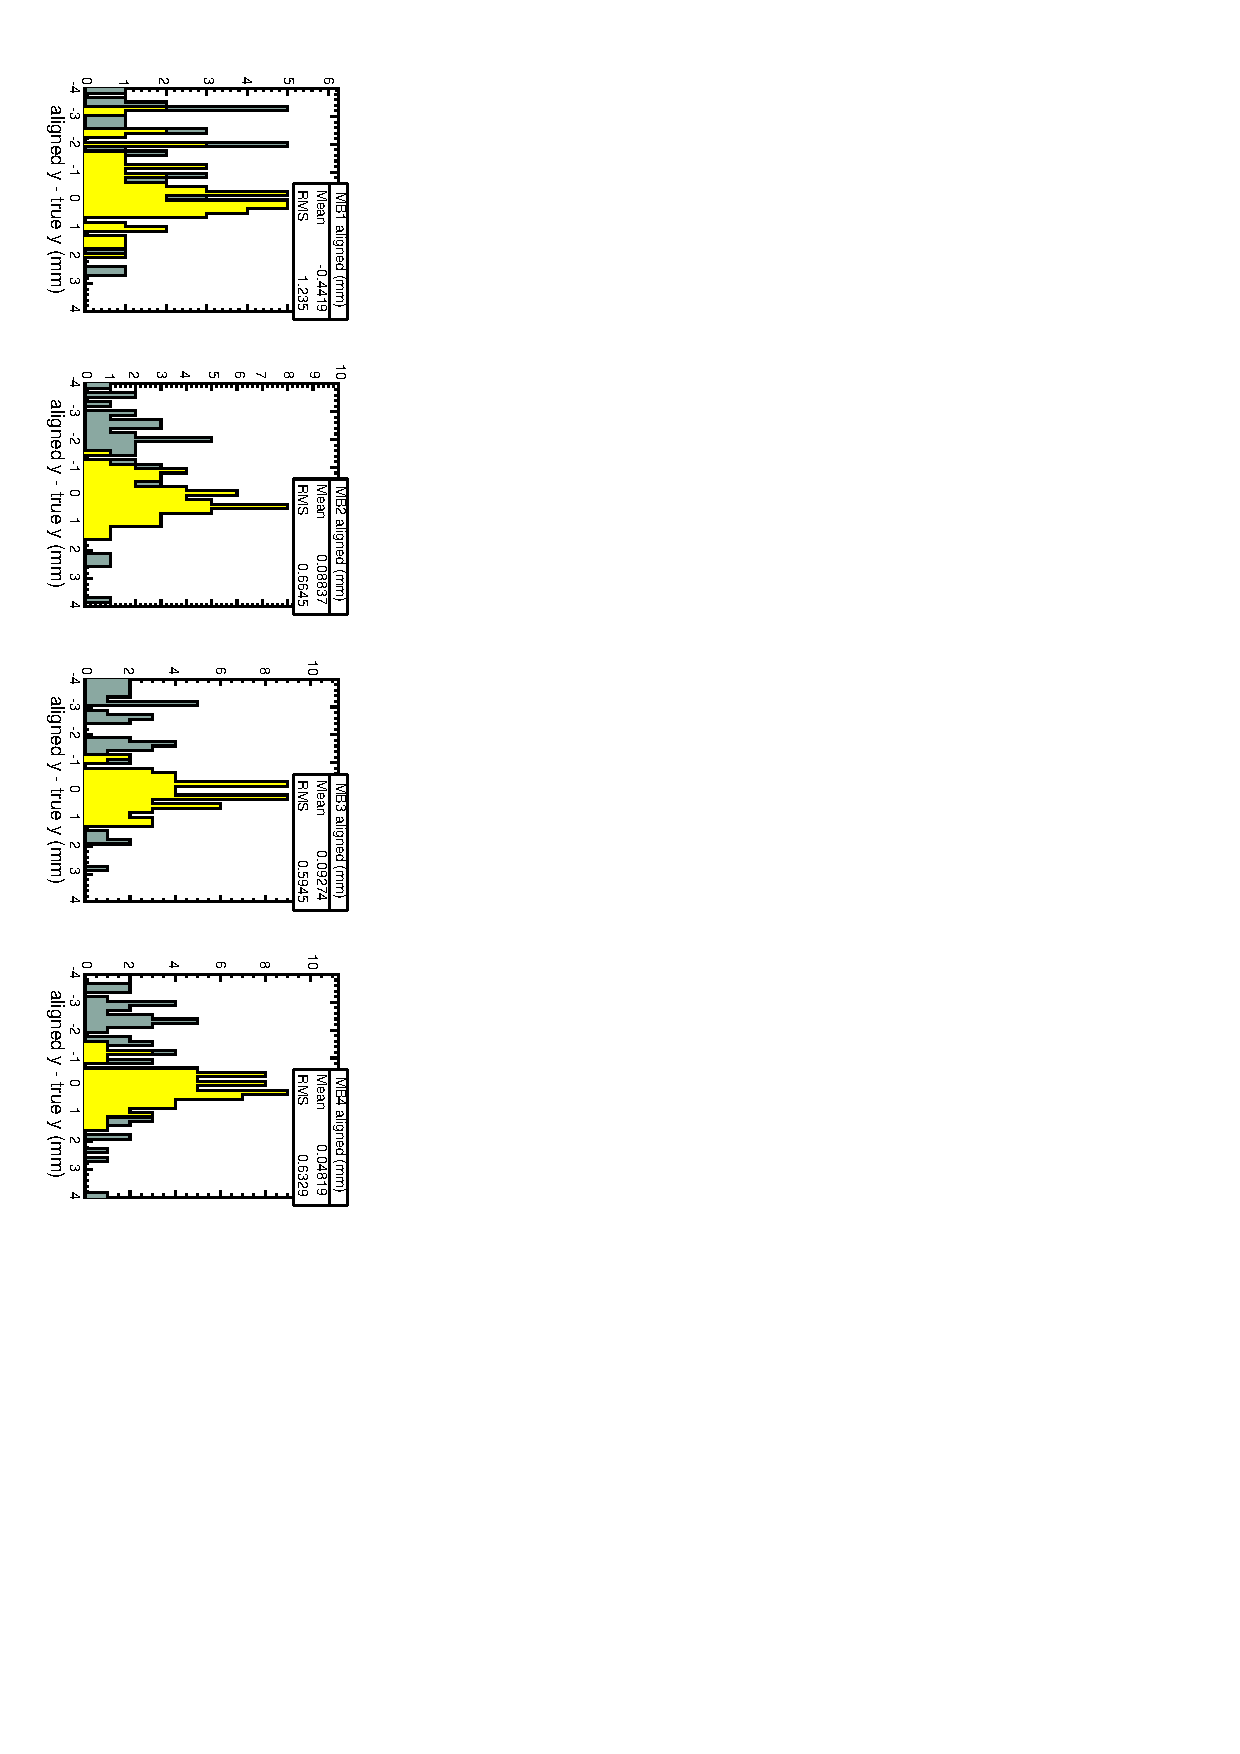
\includegraphics[height=\linewidth, angle=90]{S43_plots/MillePede_y.pdf}

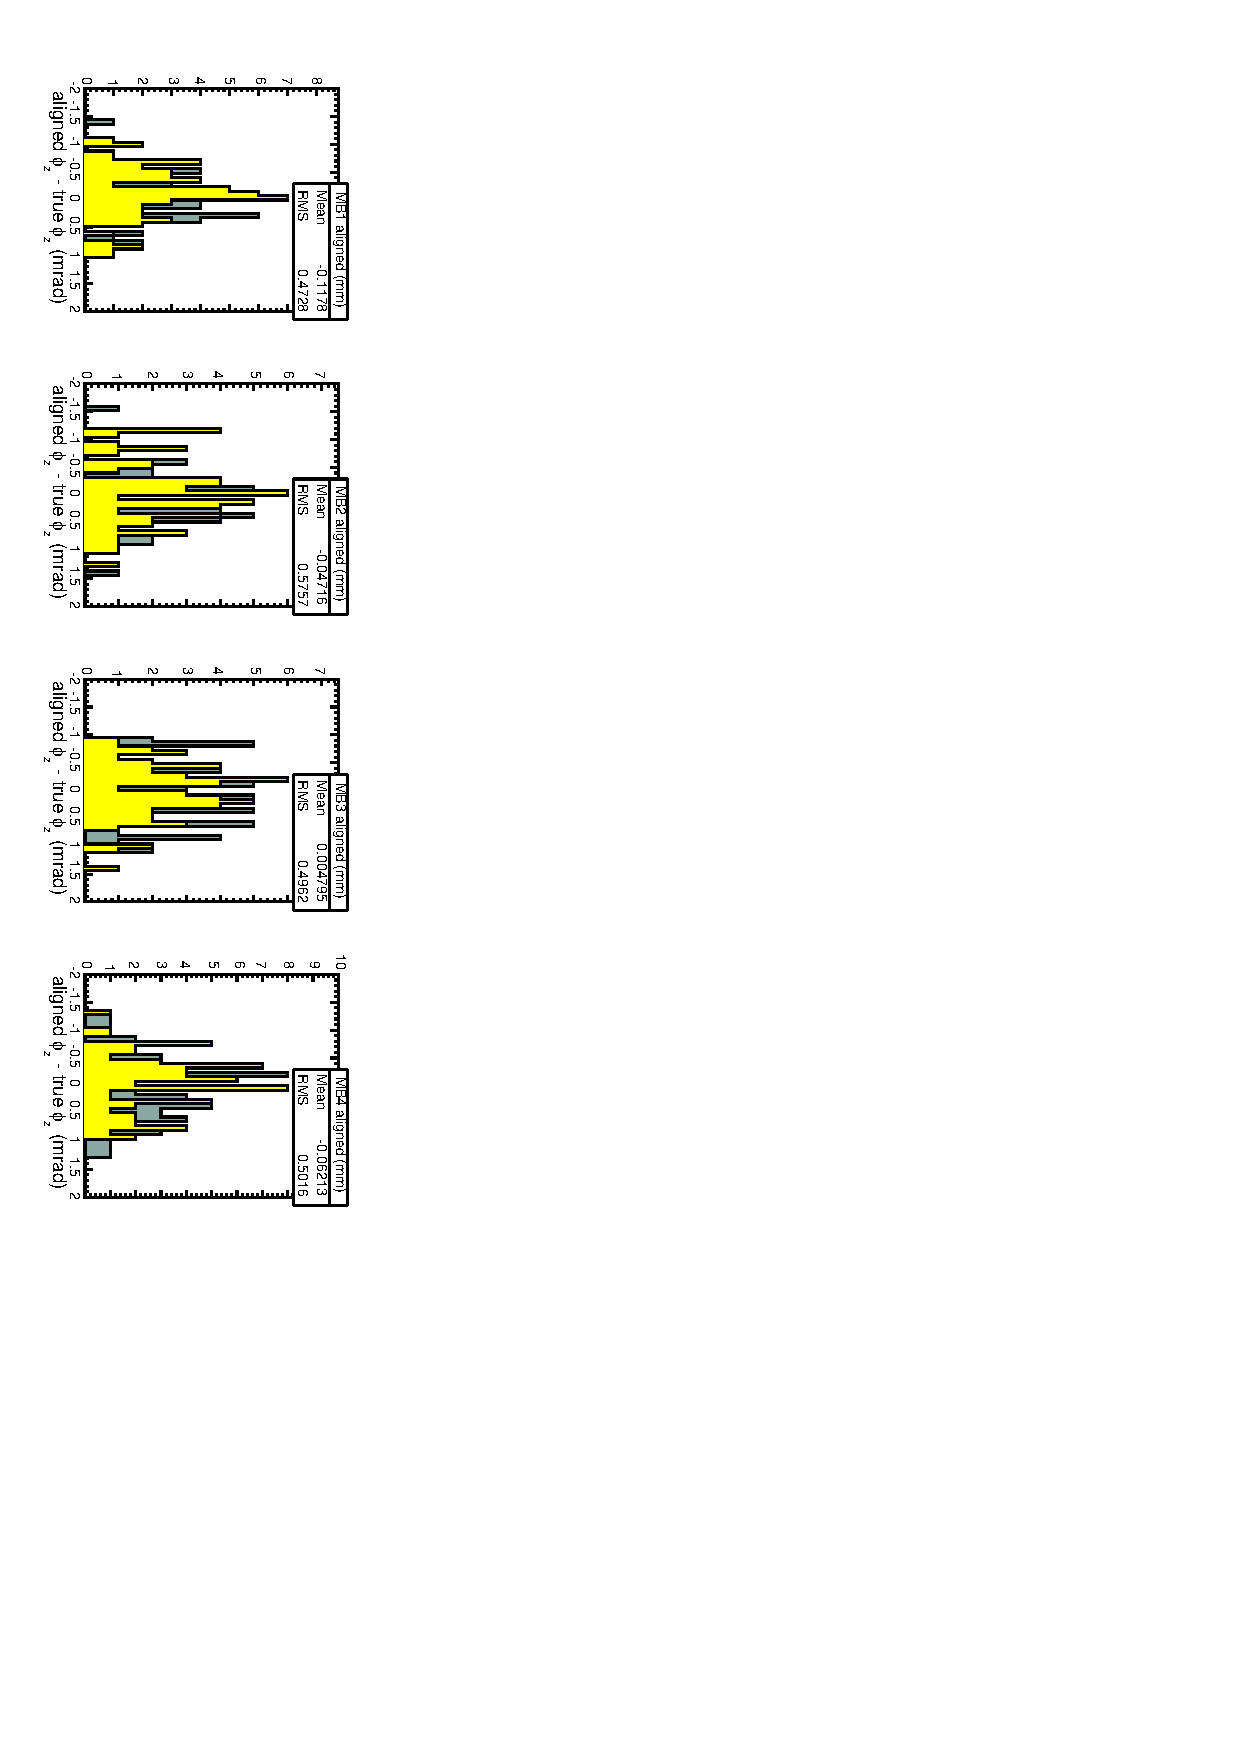
\includegraphics[height=\linewidth, angle=90]{S43_plots/MillePede_phiz.pdf}

\end{frame}

\begin{frame}
\frametitle{MillePede-survey residuals}

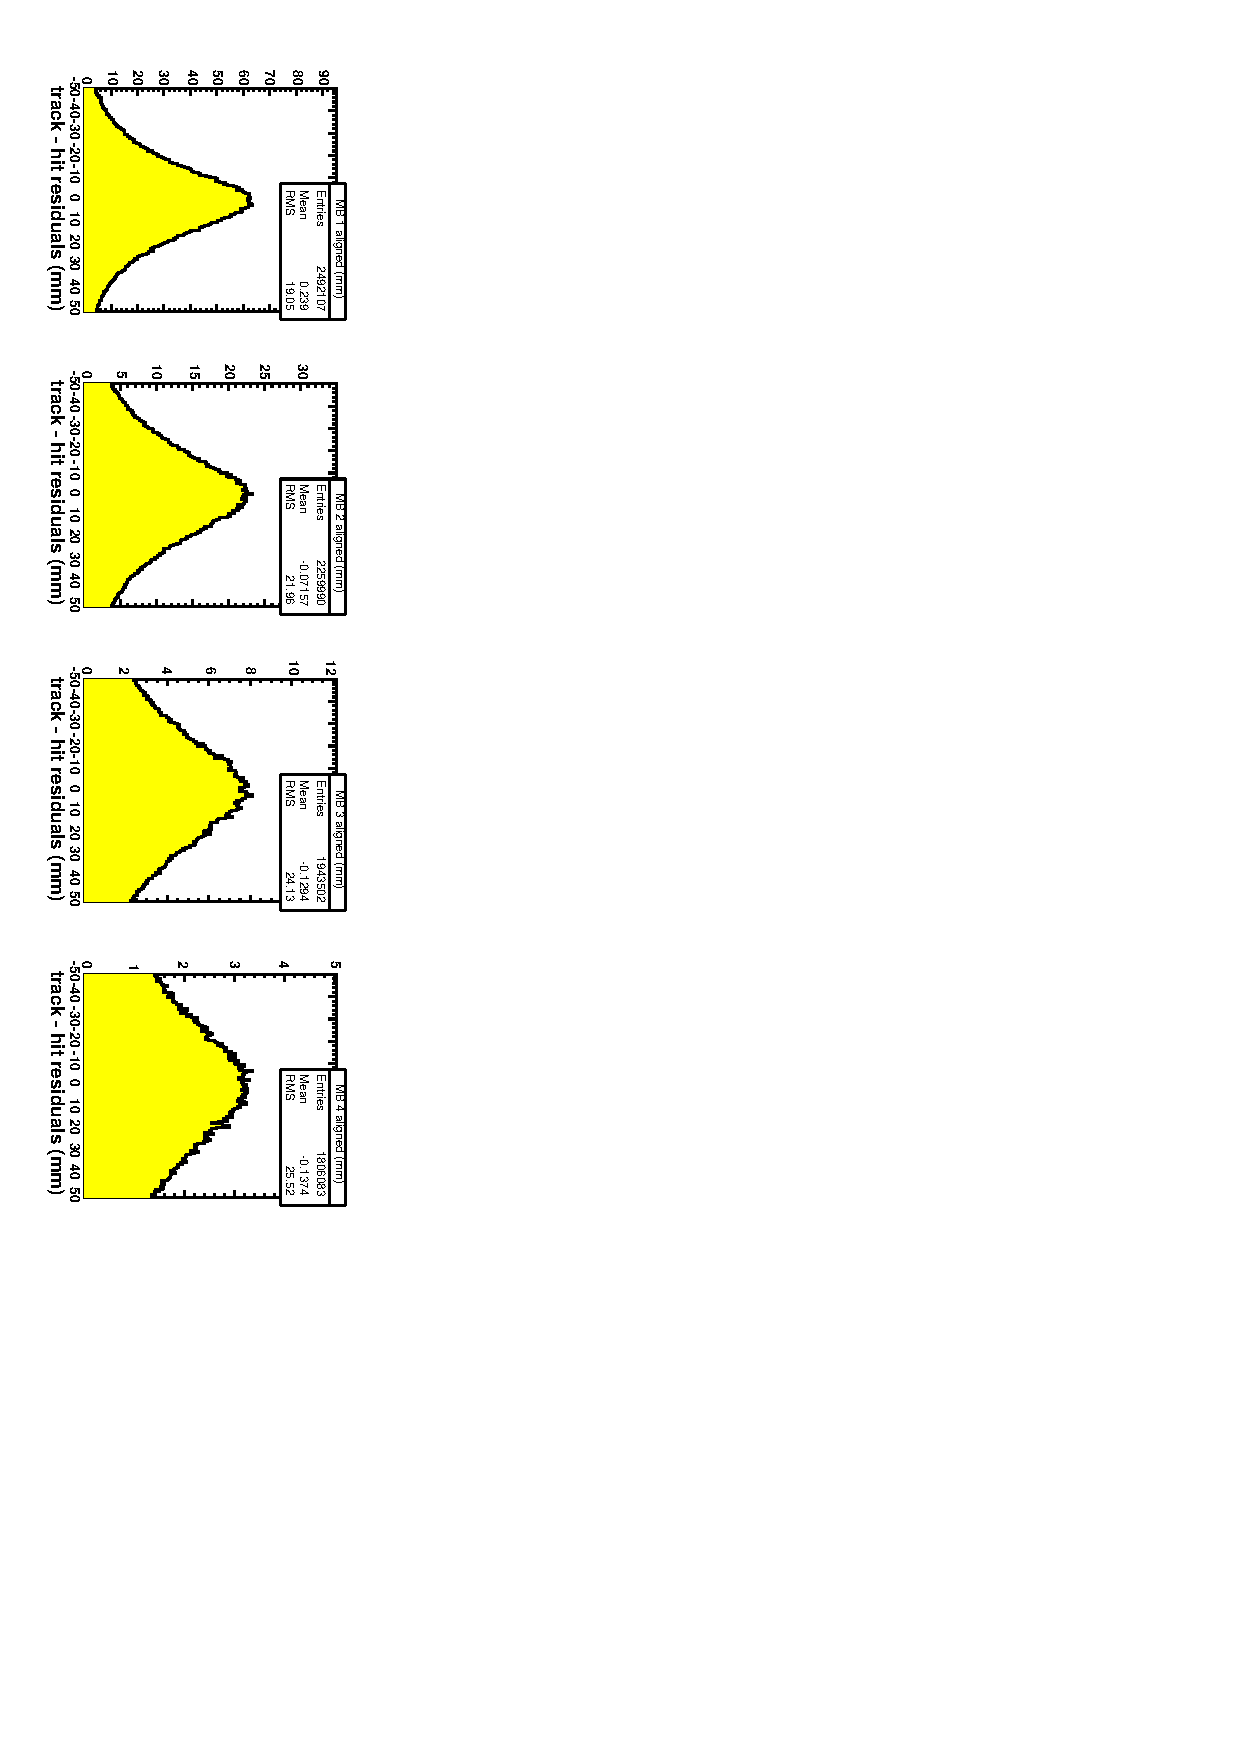
\includegraphics[height=\linewidth, angle=90]{S43_plots/RestrictPT10_MuonPT5_barrelresid.pdf}

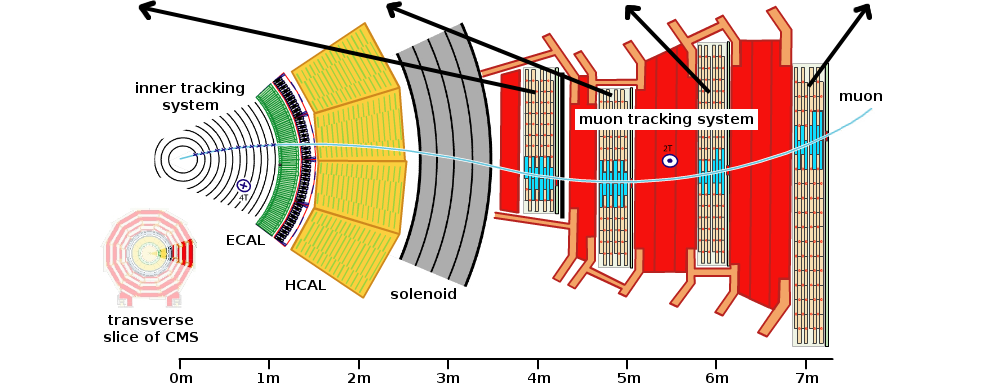
\includegraphics[width=\linewidth]{cms_slice.png}
\end{frame}

%% \begin{frame}
%% \frametitle{Outline}
%% \begin{itemize}\setlength{\itemsep}{0.75 cm}
%% \item 
%% \end{itemize}
%% %% \hspace{-0.83 cm} \textcolor{darkblue}{\Large Outline2}
%% \end{frame}

%% \section*{First section}
%% \begin{frame}
%% \begin{center}
%% \Huge \textcolor{blue}{First section}
%% \end{center}
%% \end{frame}

\end{document}
